\documentclass[conference]{IEEEtran}
\IEEEoverridecommandlockouts
% The preceding line is only needed to identify funding in the first footnote. If that is unneeded, please comment it out.

\usepackage{cite}
\usepackage{amsmath,amssymb,amsfonts}
%\usepackage{algorithmic}
\usepackage{graphicx}
\usepackage{textcomp}
\usepackage{xcolor}
\usepackage{algorithm}
\usepackage[utf8]{inputenc}
\usepackage{epstopdf}
\usepackage{caption}
\usepackage{subcaption}
\captionsetup[figure]{name={Fig.}, labelsep=period}
\captionsetup[subfigure]{labelfont=normalfont,textfont=normalfont}
%\usepackage{float}
\usepackage{amsmath, amssymb, mathtools}
\usepackage{siunitx}
\usepackage{booktabs, array, tabularx, multirow}
\usepackage{balance}
\usepackage{url}
\usepackage{enumitem}
\usepackage[font=footnotesize,labelfont=bf]{subcaption}
\usepackage{listings}
\usepackage{algpseudocode}
\usepackage{pgfplots}
\pgfplotsset{compat=1.18}
\usepackage{tikz}
\usetikzlibrary{arrows.meta, positioning, calc, shapes, fit, decorations.pathmorphing, patterns, shapes.geometric, shapes.misc, backgrounds}
\usepackage{circuitikz}
\usepackage{xcolor}
\usepackage{microtype}
\usepackage{physics}
\usepackage{bm}
\usepackage[colorlinks=true, linkcolor=blue, citecolor=blue, urlcolor=blue]{hyperref}
\usepackage{cleveref}

\usepackage{soul} %d\for highlight \hl{}

% ---------- SI units ----------
\sisetup{per-mode=symbol}
%\DeclareSIUnit{\Ah}{Ah}

%\def\BibTeX{{\rm B\kern-.05em{\sc i\kern-.025em b}\kern-.08em
%    T\kern-.1667em\lower.7ex\hbox{E}\kern-.125emX}}

    
\begin{document}

\title{Robust Evaluation of Machine Learning Models for Building Energy Consumption Prediction Under Heavy-Tailed Meter Data}

\author{\IEEEauthorblockN{Esther Omoyiwola}
\IEEEauthorblockA{\textit{Dept. of Electrical and Computer Engineering} \\
\textit{Georgia Southern University}\\
Statesboro, Georgia \\
eo03837@georgiasouthern.edu}
\and
\IEEEauthorblockN{Roland Kobla Tagayi}
\IEEEauthorblockA{\textit{Dept. of Electrical and Computer Engineering} \\
\textit{Georgia Southern University}\\
Statesboro, Georgia \\
rt10816@georgiasouthern.edu}
\and
\IEEEauthorblockN{Yvonne Okafor}
\IEEEauthorblockA{\textit{Dept. of Computer Science} \\
\textit{Georgia Southern University}\\
Statesboro, Georgia \\
yo00569@georgiasouthern.edu}
\and
\IEEEauthorblockN{Akinfenwa Ayobami}
\IEEEauthorblockA{\textit{Dept. of Mechanical Engineering} \\
\textit{Georgia Southern University}\\
Statesboro, Georgia \\
akinfenwaas@gmail.com}
\and
\IEEEauthorblockN{Vijayalakshmi Ramasamy}
\IEEEauthorblockA{\textit{Dept. of Computer Science} \\
\textit{Georgia Southern University}\\
Statesboro, Georgia \\
vramasamy@georgiasouthern.edu}
}

\maketitle

\begin{abstract}
Building energy prediction supports energy analytics, measurement and verification, demand-side management, and anomaly-aware building operation. This paper presents a comparative machine-learning study for hourly building energy meter-reading prediction using the ASHRAE Great Energy Predictor III dataset. Rather than formulating the task as conventional short-term load forecasting with autoregressive lags and fixed prediction horizons, the study treats it as a time-aware supervised prediction problem using building descriptors, meter identifiers, weather variables, and calendar features to estimate future-period hourly readings. Because the target distribution is strongly right-skewed, models are trained on $z=\log(1+y)$ and evaluated on both the logarithmic and recovered natural scales. The workflow removes known data-quality anomalies, applies memory-aware categorical encoding, uses chronological validation, and compares Linear Regression, Ridge, Lasso, XGBoost, and LightGBM. After cleaning, the final split contains about 12.68 million training observations before 1 September 2016 and 6.69 million validation observations from September to December 2016. Results show that XGBoost achieves the best root mean squared logarithmic error (RMSLE) of 1.2588 and the highest log-scale $R^2$ of 0.6364, while LightGBM is nearly tied and gives the lowest mean absolute error (MAE). Natural-scale $R^2$ remains close to zero, indicating that rare extreme readings dominate raw squared-error behavior. These findings support future meter-specific and tail-aware extensions.
\end{abstract}

\begin{IEEEkeywords}
ASHRAE energy prediction, building energy consumption, XGBoost, LightGBM, Ridge regression, Lasso regression, RMSLE, chronological validation, machine learning, gradient boosting
\end{IEEEkeywords}

\section{Introduction}
\subsection{Problem Under Study}
\IEEEPARstart{B}{uilding} energy prediction is an important problem in modern energy analytics because buildings consume a large share of electricity and thermal energy and are increasingly monitored through high-resolution meters, weather data, automation systems, and benchmarking platforms \cite{oluajayi2023datadriven,chen2025review}. Accurate prediction supports measurement and verification, fault detection, demand-side management, anomaly screening, operational planning, and performance benchmarking \cite{yesilyurt2024datadriven,mascali2023anomaly}. However, building energy prediction is challenging because real building portfolios differ in function, size, climate, site conditions, occupancy schedules, meter type, sensor quality, and operating behavior. These differences produce hourly meter readings with long periods of normal consumption and occasional extreme values, creating a heavy-tailed target distribution that can distort raw squared-error metrics. Although physics-based and calibrated engineering models remain useful when detailed building information is available, large portfolios often lack complete and consistent physical data. This has increased the use of data-driven models that learn directly from historical meter readings, weather variables, calendar features, building descriptors, and operational information \cite{chen2025review,yesilyurt2024datadriven}.

\subsection{Related Work}
Several review studies show that data-driven building energy prediction is not defined by one preferred algorithm. Instead, performance depends on the interaction among data granularity, building type, target variable, feature engineering, preprocessing, validation strategy, and evaluation metric. Amasyali and El-Gohary reviewed data-driven building energy consumption prediction studies and emphasized prediction scope, data properties, preprocessing methods, algorithms, and performance measures as major sources of variation \cite{amasyali2018review}. Wei et al. surveyed data-driven approaches for both prediction and classification in building energy analysis, covering statistical regression, artificial neural networks, support vector machines, decision trees, clustering methods, and other learning approaches across different building archetypes and granularities \cite{wei2018review}. Bourdeau et al. further emphasized that input-data characteristics, preprocessing choices, energy end-use, building typology, forecasting horizon, and accuracy assessment strongly influence reported model performance \cite{bourdeau2019review}. These findings directly support the present study's decision to treat preprocessing, target transformation, and validation design as central methodological components rather than secondary implementation details.

Recent studies also show that building load prediction has become a mature but still methodologically uneven field. Zhang et al. reviewed machine-learning applications in building load prediction and organized the field around the machine-learning elements of task, performance, and experience, making clear that model evaluation must be tied to the prediction objective and available data structure \cite{zhang2021review}. Khalil et al. reviewed machine-learning, deep-learning, and statistical methods for building energy consumption forecasting and highlighted the importance of data availability, preprocessing, model selection, and application context \cite{khalil2022review}. These reviews collectively indicate that the strongest building energy prediction studies are not those that simply apply a complex algorithm, but those that align the problem formulation, data treatment, model class, and evaluation metric with the physical and statistical structure of the task.

Linear and regularized linear models provide important baselines for this study because they establish whether the selected building, weather, calendar, and meter-related predictors contain useful global linear structure. Ordinary Linear Regression offers a transparent additive reference model, while Ridge Regression improves coefficient stability under multicollinearity through an $\ell_2$ penalty \cite{hoerl1970ridge}, and Lasso Regression introduces an $\ell_1$ penalty that can shrink selected coefficients to zero and support sparse feature selection \cite{tibshirani1996lasso}. However, these models remain limited for heterogeneous building energy data because they assume a relatively smooth and global relationship between predictors and the response, whereas actual meter readings may vary nonlinearly across sites, meter types, operating schedules, weather regimes, and primary-use categories. Gradient boosting provides a more flexible alternative by building an additive ensemble of decision trees that sequentially reduce prediction error \cite{friedman2001greedy}. XGBoost extends this framework through regularized scalable tree boosting, sparsity-aware learning, and efficient tree construction \cite{chen2016xgboost}, while LightGBM further improves computational efficiency using histogram-based learning and leaf-wise tree growth \cite{ke2017lightgbm}. These characteristics make boosted-tree models well suited for large, nonlinear, and interaction-heavy building energy datasets. Therefore, the gap addressed in this study is the development of a fair, reproducible, and scale-aware comparative framework that tests whether XGBoost and LightGBM provide a meaningful advantage over linear and regularized baselines when all models are trained under the same preprocessing, chronological validation, and log-target evaluation design. 

The ASHRAE Great Energy Predictor III dataset provides a strong basis for this study because it was developed from the Building Data Genome Project 2, a large collection of non-residential building meter data with building metadata and weather observations \cite{miller2020bdg2}. The ASHRAE GEPIII competition further demonstrated the practical relevance of this prediction problem by challenging participants to estimate metered building energy use across electricity, chilled water, steam, and hot-water meters \cite{miller2020ashrae}. The dataset is valuable precisely because it resembles real energy analytics conditions: it contains heterogeneous buildings, multiple sites, missing metadata, weather variation, categorical structure, known anomalies, and a highly skewed target distribution. These properties make the dataset useful for benchmarking machine-learning models, but they also make careless validation or metric selection risky. This study then examines whether hourly building energy meter readings from the ASHRAE Great Energy Predictor III dataset can be predicted reliably using a time-aware, log-scale supervised regression framework. Instead of treating the problem as a full short-term load forecasting task with explicit lagged-load variables and fixed forecast horizons, the study evaluates how well Linear Regression, Ridge Regression, Lasso Regression, XGBoost, and LightGBM predict future-period meter readings under the same preprocessing and chronological validation design. 

\subsection{Research Questions and Contributions of the Study}
The main research questions are whether nonlinear ensemble models outperform linear and regularized linear baselines, whether the log-transformed target $z=\log(1+y)$ provides a more stable representation of the highly skewed meter-reading distribution, and how natural-scale metrics, log-scale metrics, and actual-versus-predicted diagnostics jointly explain model performance. Given the state-of-the-art research reviewed earlier, the salient contributions of this paper are as follows.
\begin{itemize}
\item This work presents a unified comparison of Linear Regression, Ridge Regression, Lasso Regression, XGBoost, and LightGBM under the same preprocessing, feature construction, target transformation, and chronological validation framework. 
\item It applies a scale-aware modeling strategy using $z=\log(1+y)$ to handle the strongly right-skewed meter-reading distribution.
\item The study interprets model performance using both natural-scale and log-scale metrics, including mean absolute error (MAE) and root mean square error (RMSE), RMSLE, $R^{2}$, $R^{2}_{\log}$, and actual-versus-predicted diagnostics. 
\end{itemize}

The remainder of this paper is organized as follows. Section II describes the ASHRAE dataset, preprocessing steps, feature groups, data-quality filtering, and assumptions used in the study. Section III presents the mathematical formulation of the supervised log-scale prediction problem, the five model objectives, the chronological validation design, and the evaluation metrics. Section IV reports the empirical results, including aggregate error metrics and actual-versus-predicted diagnostics on both natural and logarithmic scales. Section V discusses the interpretation of the results, the reasons for the stronger performance of boosted trees, the limitations of natural-scale metrics under heavy-tailed targets, and the practical implications for deployment. Section VI concludes the paper and identifies future work needed to extend the current framework into a full operational forecasting system.

\section{Dataset Description and Exploratory Analysis}
This study uses the ASHRAE Great Energy Predictor III dataset, a large-scale building energy dataset associated with the Building Data Genome Project 2. The merged data include hourly meter readings, building metadata, and weather observations for 1,449 buildings across 16 sites from 1 January to 31 December 2016, producing 20,216,100 raw observations after integrating the meter, building, and weather tables. The prediction target is \texttt{meter\_reading}, which represents multiple meter categories, including electricity, chilled water, steam, and hot water; therefore, natural-scale errors are reported in original meter-reading units rather than treated as one universal physical unit. To prepare the model-ready dataset, known data-quality issues, nonfinite values, six unreliable building identifiers, and the early electricity-meter zero anomaly before 20 May 2016 were removed. A chronological split was then used, with observations before 1 September 2016 assigned to training and observations from September through December assigned to validation, as summarized in Table~\ref{tab:dataset_summary}. This design better represents future-period prediction than random splitting because it avoids leakage of seasonal and operational information across training and validation sets. The final feature set combines building, meter, and site identifiers; weather variables such as air temperature, cloud coverage, dew temperature, precipitation, and wind direction; calendar variables such as hour, day of week, day, year, and weekend indicator; log-transformed building area; and one-hot encoded primary-use categories.
\begin{table}[!t]
\centering
\caption{Dataset and Validation Summary.}
\label{tab:dataset_summary}
\begin{tabular}{p{0.52\linewidth}p{0.36\linewidth}}
\toprule
\textbf{Item} & \textbf{Value} \\
\midrule
Raw Merged Observations & 20,216,100 \\
Buildings & 1,449 \\
Sites & 16 \\
Observation Period & 1 Jan.--31 Dec. 2016 \\
Temporal Resolution & Hourly \\
Target Variable & \texttt{meter\_reading} \\
Transformed Target & $z=\log(1+y)$ \\
Training Period & Jan.--Aug. 2016 \\
Validation Period & Sept.--Dec. 2016 \\
Training Observations After Filtering & 12,675,376 \\
Validation Observations After Filtering & 6,685,946 \\
Models Evaluated & Linear, Ridge, Lasso, XGBoost, LightGBM \\
\bottomrule
\end{tabular}
\end{table}

Exploratory analysis confirmed that the target distribution is strongly right-skewed, with many observations near zero and a much smaller number of very large readings. Fig.~\ref{fig:target_distribution} therefore provides direct justification for the log-scale modeling strategy used in this study. The raw distribution shows the heavy-tailed nature of the original meter readings, while the transformed distribution shows a more stable response scale for model fitting.
\begin{figure}[!t]
\centering
\begin{subfigure}[t]{\columnwidth}
    \centering
    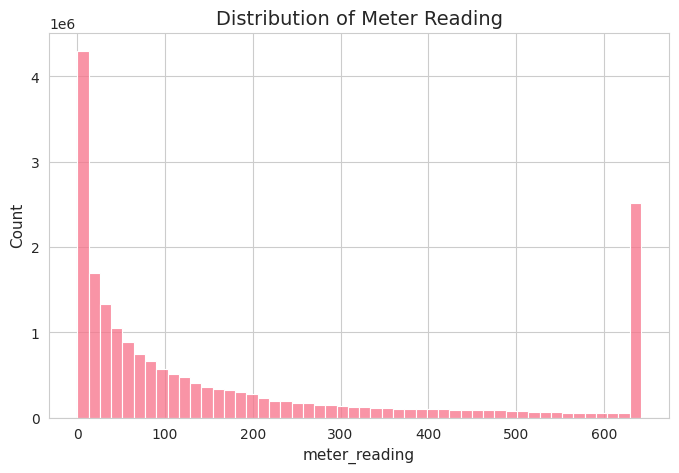
\includegraphics[width=1\columnwidth]{raw_meter_reading_hist.png}
    \caption{\small{Raw meter-reading distribution.}}
    \label{fig:raw_meter_reading_hist}
\end{subfigure}
\vspace{0.8ex}
\begin{subfigure}[t]{\columnwidth}
    \centering
    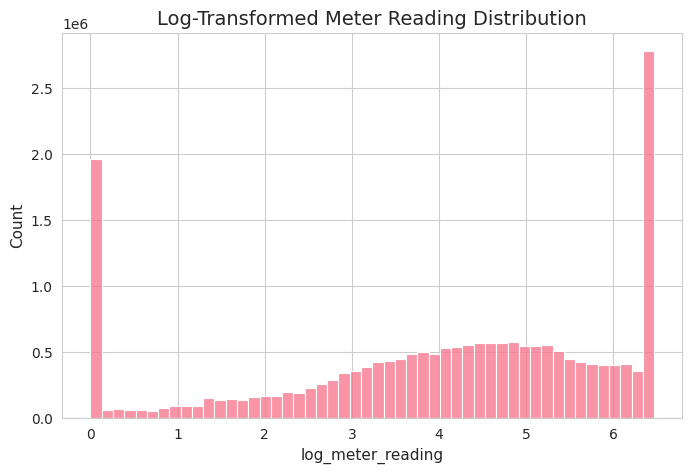
\includegraphics[width=1\columnwidth]{log_meter_reading_hist.png}
    \caption{\small{Log-transformed meter-reading distribution.}}
    \label{fig:log_meter_reading_hist}
\end{subfigure}
\caption{\small{Target-variable distribution before and after logarithmic transformation. The raw meter readings are heavily right-skewed, while $\log(1+y)$ compresses the extreme upper tail and provides a more stable modeling target.}}
\label{fig:target_distribution}
\end{figure}
The correlation analysis in Fig. \ref{fig:corr_heatmap} shows that individual numerical predictors have weak linear correlation with the raw meter readings. This does not mean the predictors are unimportant; rather, it suggests that building energy use is governed by nonlinear and conditional relationships involving building type, time, weather, site, and meter category. The stronger correlation between air temperature and dew temperature also indicates that some weather variables are mutually related, which supports the use of models that can tolerate correlated predictors.
\begin{figure}[!t]
    \centering
    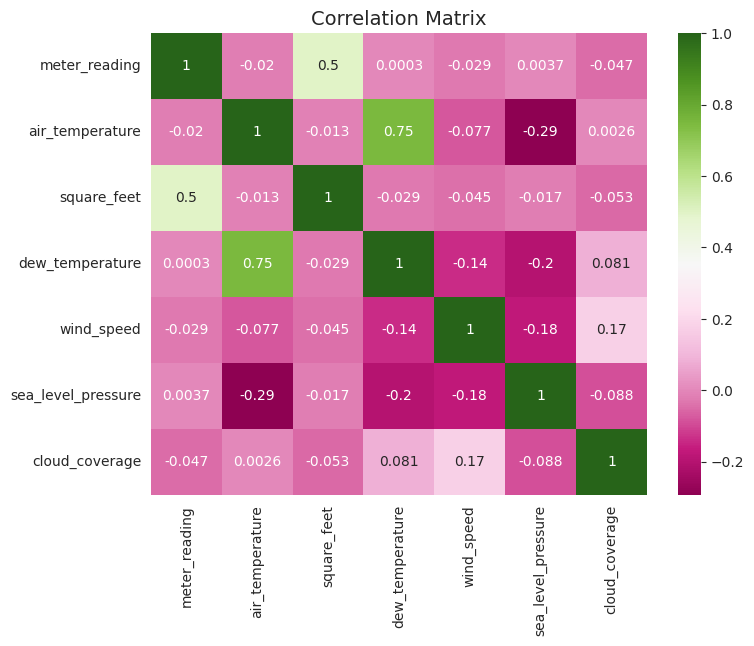
\includegraphics[width=1\columnwidth]{correlation_heatmap.png}
    \caption{\small{Correlation matrix of selected numerical variables. The weak linear association between individual predictors and meter readings suggests that nonlinear models are needed, while stronger relationships among weather variables indicate possible meteorological collinearity.}}
    \label{fig:corr_heatmap}
\end{figure}
Temporal aggregation provides one of the clearest signals in the data. As shown in Fig. \ref{fig:temporal_patterns}, average energy use varies by hour of day, day of week, and across the annual timeline. The hourly and weekly profiles support the inclusion of calendar variables, while the annual trend confirms that energy use changes over time rather than behaving as an independently distributed response.
\begin{figure}[!t]
\centering
\begin{subfigure}[t]{\columnwidth}
    \centering
    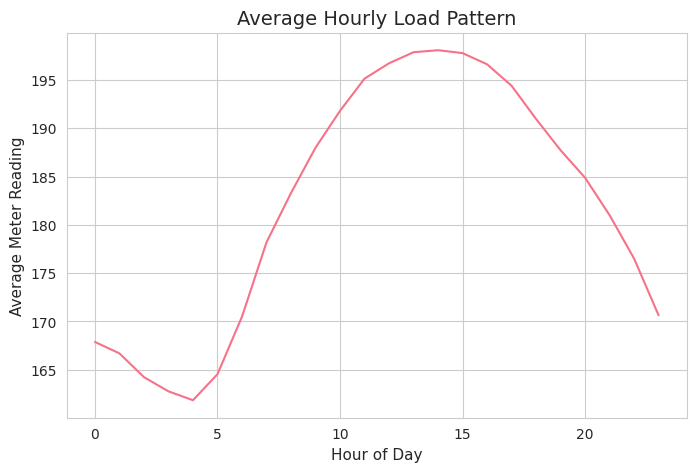
\includegraphics[width=1\columnwidth]{hourly_load_profile.png}
    \caption{\small{Average meter reading by hour of day.}}
    \label{fig:hourly_load_profile}
\end{subfigure}
\vspace{0.8ex}
\begin{subfigure}[t]{\columnwidth}
    \centering
    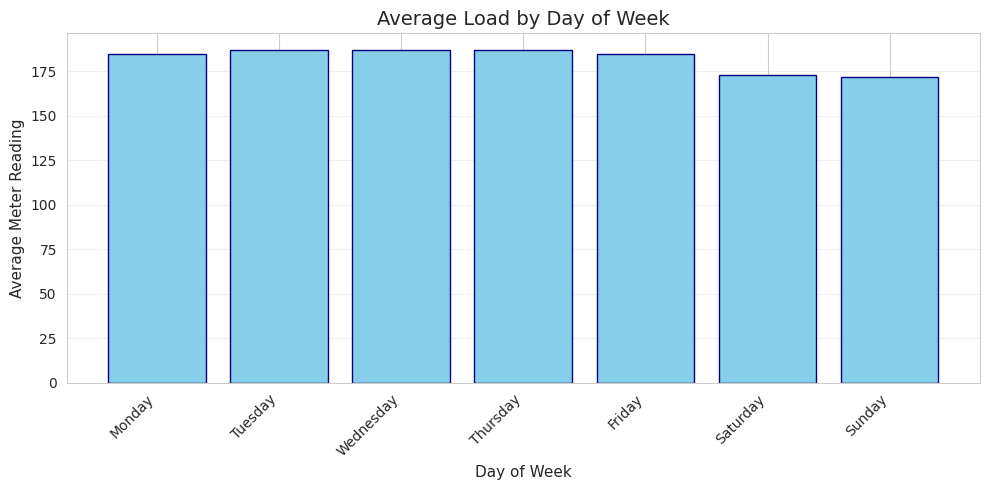
\includegraphics[width=1\columnwidth]{weekday_load_profile.png}
    \caption{\small{Average meter reading by day of week.}}
    \label{fig:weekday_load_profile}
\end{subfigure}
\vspace{0.8ex}
\begin{subfigure}[t]{\columnwidth}
    \centering
    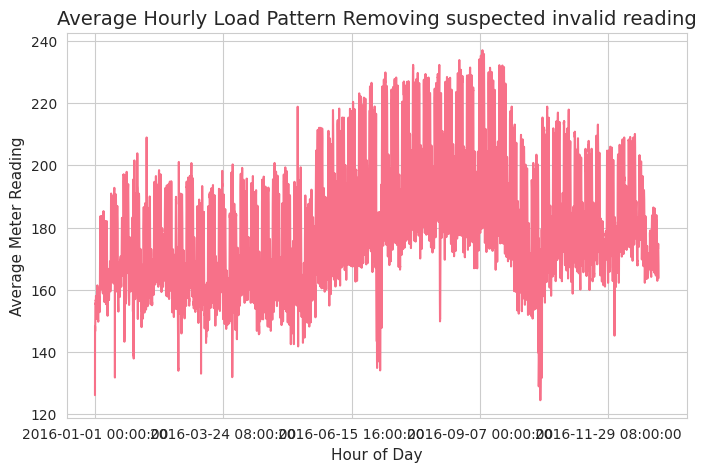
\includegraphics[width=1\columnwidth]{yearly_load_trend.png}
    \caption{\small{Average meter reading across the full year.}}
    \label{fig:yearly_load_trend}
\end{subfigure}
\caption{\small{Temporal patterns in the ASHRAE meter readings. The profiles show daily, weekly, and annual structure, justifying the use of chronological validation and calendar-based predictors.}}
\label{fig:temporal_patterns}
\end{figure}
Finally, the meter-type summary in Table \ref{tab:meter_type_summary} is retained because the target variable is not physically homogeneous. Electricity, chilled water, steam, and hot-water readings can have different scales and operating patterns. This justifies retaining \texttt{meter} as a predictor and explains why model performance should be interpreted carefully on the natural meter-reading scale.
\begin{table}[!t]
\centering
\caption{Meter-type summary used to interpret the response variable.}
\label{tab:meter_type_summary}
\begin{tabular}{lccc}
\toprule
\textbf{Meter Type} & \textbf{Meter ID} & \textbf{Total Readings} & \textbf{Median Reading} \\
\midrule
Electricity   & 0 & 12,060,910 & 62.84375 \\
Chilled Water & 1 & 4,182,440  & 120.50000 \\
Steam         & 2 & 2,708,713  & 257.75000 \\
Hot Water     & 3 & 1,264,037  & 39.62500 \\
\bottomrule
\end{tabular}
\end{table}
Overall, the exploratory analysis supports three modeling decisions used in this study. First, the strong skewness of the response justifies the log-transformed target. Second, temporal, building, meter, and weather variables should be retained because the data show clear time structure and heterogeneous operating conditions. Third, model evaluation must use both log-scale and natural-scale metrics, since ordinary operating behavior and rare extreme meter readings represent different aspects of predictive performance.

\section{Mathematical Modeling and Evaluation Framework}
Fig. \ref{fig:Framework1} summarizes the complete research workflow used for building energy prediction. The process begins with raw ASHRAE meter, building, and weather data, then applies data-quality filtering, feature construction, and log-based target formulation to prepare the dataset for modeling. A chronological train--validation split is used to preserve the time structure of the data, after which five regression models are trained and evaluated using both natural-scale and log-scale performance metrics. The final stages compare model behavior through diagnostic plots and error analysis to identify the best-performing approach and derive practical insights from the results.
\begin{figure*}[!t]
\centering
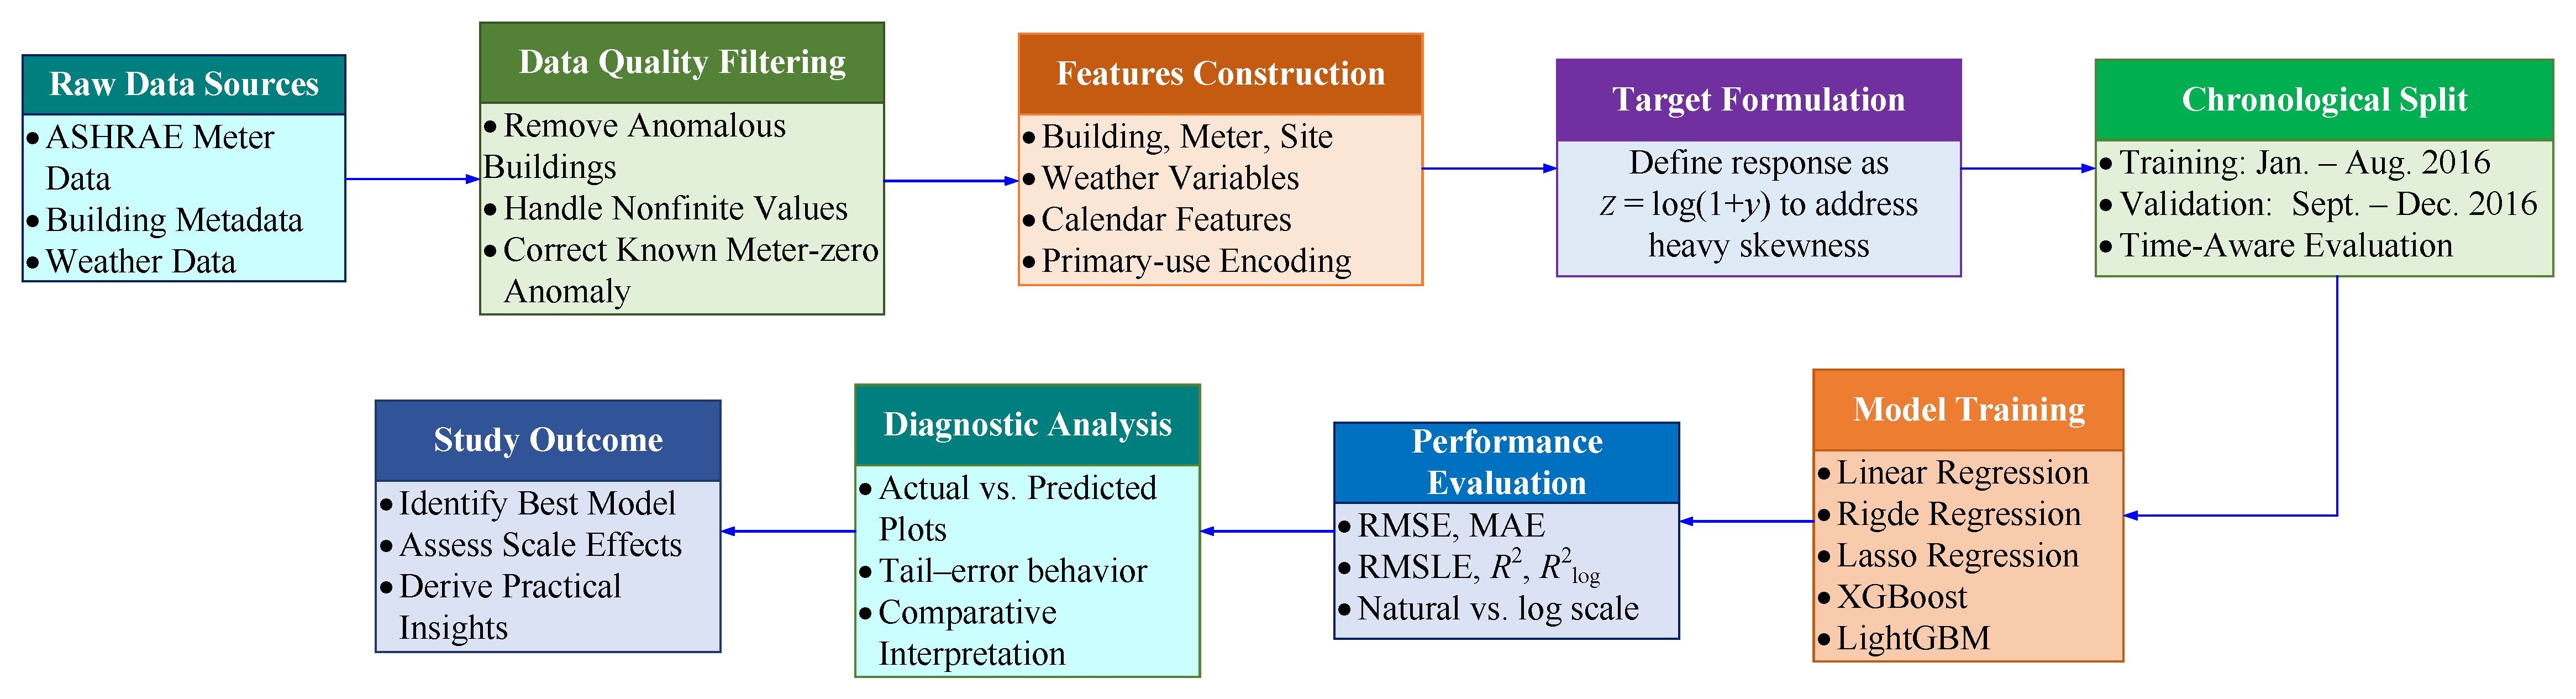
\includegraphics[width=2\columnwidth]{Framework1.pdf}
\caption{\small{Research workflow: The study begins with raw ASHRAE meter, building, and weather data, followed by data-quality filtering, feature construction, log-target formulation, chronological train--validation splitting, five-model training, multi-scale evaluation, and diagnostic interpretation.}}
\label{fig:Framework1}
\end{figure*}

\subsection{Supervised Regression Formulation}
Let $\mathcal{D}=\{(\mathbf{x}_i,y_i,t_i)\}_{i=1}^{N}$ denote the dataset, where $\mathbf{x}_i\in\mathbb{R}^{p}$ is the feature vector, $y_i\geq0$ is the observed meter reading, and $t_i$ is the timestamp. The prediction objective is to learn a function $f:\mathbb{R}^{p}\rightarrow\mathbb{R}$ such that $\hat{z}_i = f(\mathbf{x}_i), z_i = \log(1+y_i)$. The recovered natural-scale prediction is $\hat{y}_i=\max\left\{\exp(\hat{z}_i)-1,0\right\}$. The maximum operation enforces the physical nonnegativity of meter readings.

\subsection{Linear Regression}
Ordinary least-squares linear regression assumes a global additive relationship described by $\hat{z}_i = \beta_0+\mathbf{x}_i^T\boldsymbol{\beta}.$ The parameters are obtained by minimizing $\min_{\beta_0,\boldsymbol{\beta}}
    \sum_{i\in\mathcal{T}}
    \left(z_i-\beta_0-\mathbf{x}_i^T\boldsymbol{\beta}\right)^2$, where $\mathcal{T}$ is the training index set. This model is interpretable but cannot naturally represent nonlinear thresholds or high-order interactions unless they are manually engineered.

\subsection{Lasso Regression}
Lasso regression modifies the linear regression objective by solving the $\ell_1$-penalized problem $\min_{\beta_0,\boldsymbol{\beta}}\{(1/2n)\mathrm{RSS}+\lambda_1\|\boldsymbol{\beta}\|_1\}$, where RSS denotes the training residual sum of squares. The $\ell_1$ penalty can shrink selected coefficients exactly to zero, which supports sparse feature representation. The final Lasso model uses $\lambda_1=0.0100131$.

\subsection{Ridge Regression}
Ridge regression extends the linear regression objective by minimizing the residual sum of squares (RSS) with an added $\ell_2$ penalty, written compactly as $\mathrm{RSS}+\lambda_2\|\boldsymbol{\beta}\|_2^2$. The penalty parameter $\lambda_2>0$ shrinks the regression coefficients and improves numerical stability when predictors are correlated. In this study, $\lambda_2=0.100266$ was used for final Ridge training.

\subsection{Gradient-Boosted Decision Trees}
Gradient boosting represents the prediction function as an additive ensemble defined by
\begin{equation}
    \hat{z}_i^{(K)}=\sum_{k=1}^{K}\eta f_k(\mathbf{x}_i),
    \label{eq:gb_additive}
\end{equation}
where $f_k$ is a regression tree and $\eta$ is the learning rate. Each new tree is fitted to reduce the objective
\begin{equation}
    \mathcal{L}^{(K)} =
    \sum_{i\in\mathcal{T}}
    \ell\left(z_i,\hat{z}_i^{(K)}\right)
    +\sum_{k=1}^{K}\Omega(f_k),
    \label{eq:gb_objective}
\end{equation}
where $\ell(\cdot)$ is the loss function and $\Omega(f_k)$ is a complexity penalty. XGBoost uses a regularized objective of the form
\begin{equation}
    \Omega(f)=\gamma T+\frac{1}{2}\lambda\sum_{j=1}^{T}w_j^2,
    \label{eq:xgb_complexity}
\end{equation}
where $T$ is the number of leaves and $w_j$ is the score assigned to leaf $j$. Using a second-order Taylor approximation, the split gain can be expressed as
$    \mathcal{G}_{split}
    =
    \frac{1}{2}\left[
    \frac{G_L^2}{H_L+\lambda}
    +
    \frac{G_R^2}{H_R+\lambda}
    -
    \frac{(G_L+G_R)^2}{H_L+H_R+\lambda}
    \right]-\gamma,$ where $G$ and $H$ denote sums of first- and second-order gradients for candidate child nodes. LightGBM follows the same broad gradient-boosting principle but uses efficient histogram-based split search and leaf-wise growth strategies to improve computational efficiency for large datasets.

\subsection{Log-Scale Error Interpretation}
The RMSLE metric used in this study is expressed as
\begin{equation}
    \mathrm{RMSLE}
    =
    \sqrt{
    \frac{1}{n}
    \sum_{i=1}^{n}
    \left[
    \log(1+\hat{y}_i)-\log(1+y_i)
    \right]^2
    }.
    \label{eq:rmsle}
\end{equation}
Since $\hat{z}_i=\log(1+\hat{y}_i)$ and $z_i=\log(1+y_i)$, RMSLE is identical to RMSE on the log target.

\textit{Proposition 1}: For positive readings, log-scale error approximates multiplicative relative error when prediction error is moderate. \noindent\emph{Proof:} Let $\delta_i=\frac{\hat{y}_i-y_i}{1+y_i}$. Then
$    \hat{z}_i-z_i
    =\log(1+\hat{y}_i)-\log(1+y_i) \nonumber
    =\log\left(\frac{1+\hat{y}_i}{1+y_i}\right) \nonumber
    =\log(1+\delta_i).$ For $|\delta_i|<1$, the Taylor expansion gives
$    \log(1+\delta_i)=\delta_i-\frac{\delta_i^2}{2}+\frac{\delta_i^3}{3}-\cdots.$ Thus, to first order, $\hat{z}_i-z_i\approx \delta_i$. Squared log error, therefore, penalizes approximate multiplicative error rather than raw absolute error. This proves why RMSLE is less dominated by large absolute readings than natural-scale RMSE. 

\subsection{Chronological Validation}
Let the cutoff time be $t_c=$ 1 September 2016. The training and validation sets are $\mathcal{T}=\{i:t_i<t_c\},\mathcal{V}=\{i:t_i\geq t_c\}$.
The study uses an expanding-window split in which each fold trains on all observations up to a time boundary and validates on the next chronological block as shown in Table \ref{tab:cv}.

\begin{table}[!t]
\caption{Chronological Expanding-Window Validation Blocks}
\label{tab:cv}
\centering
\begin{tabular}{lll}
\toprule
\textbf{Fold} & \textbf{Training Window Ends} & \textbf{Validation Window} \\
\midrule
1 & 20 Mar. 2016 & 20 Mar.--2 Jun. 2016 \\
2 & 2 Jun. 2016 & 2 Jun.--12 Aug. 2016 \\
3 & 12 Aug. 2016 & 12 Aug.--22 Oct. 2016 \\
4 & 22 Oct. 2016 & 22 Oct.--31 Dec. 2016 \\
\bottomrule
\end{tabular}
\end{table}

\textit{Proposition 2}: The chronological split prevents future validation timestamps from being used in model fitting.

\textit{Proof}: By construction, every training observation satisfies $t_i<t_c$, and every validation observation satisfies $t_i\geq t_c$. Therefore, no validation timestamp can appear in the training index set. Since the fitted model parameters are estimated only over $\mathcal{T}$, the final holdout represents a future-period test relative to the training period.

\subsection{Evaluation Metrics}
The original-scale metrics are
\begin{align}
    \mathrm{RMSE} &=
    \sqrt{\frac{1}{n}\sum_{i=1}^{n}(y_i-\hat{y}_i)^2}, \label{eq:rmse}\\
    \mathrm{MAE} &=
    \frac{1}{n}\sum_{i=1}^{n}|y_i-\hat{y}_i|, \label{eq:mae}\\
    R^2 &=
    1-\frac{\sum_{i=1}^{n}(y_i-\hat{y}_i)^2}
    {\sum_{i=1}^{n}(y_i-\bar{y})^2}. \label{eq:r2}
\end{align}
The log-scale explained variance is
\begin{equation}
    R^2_{\log}
    =
    1-\frac{\sum_{i=1}^{n}(z_i-\hat{z}_i)^2}
    {\sum_{i=1}^{n}(z_i-\bar{z})^2}.
    \label{eq:r2log}
\end{equation}
Using both $R^2$ and $R^2_{\log}$ is necessary because the original target has extreme upper-tail observations, while the log target measures the dominant structure of ordinary building operation more clearly. Table \ref{tab:parameters} shows a summary of the quantities derived from the data set, the hyperparameters selected by the model, and the assumptions used in this study.
\begin{table}[!t]
\centering
\caption{Dataset Quantities and Model Hyperparameters}
\label{tab:parameters}
\footnotesize
\setlength{\tabcolsep}{4pt}
\renewcommand{\arraystretch}{1.12}
\begin{tabular}{@{}p{0.58\columnwidth}p{0.34\columnwidth}@{}}
\toprule
\textbf{Quantity} & \textbf{Value} \\
\midrule
\multicolumn{2}{@{}l}{\textit{Dataset and validation design}} \\
Raw merged observations & 20,216,100 \\
Final training observations & 12,675,376 \\
Final validation observations & 6,685,946 \\
Validation cutoff & 1 Sept. 2016 \\
Target transformation & $\log(1+y)$ \\
\midrule
\multicolumn{2}{@{}l}{\textit{Linear-model hyperparameters}} \\
Ridge penalty & $\lambda_2=0.100266$ \\
Lasso penalty & $\lambda_1=0.0100131$ \\
\midrule
\multicolumn{2}{@{}l}{\textit{Boosting-model hyperparameters}} \\
XGBoost learning rate & 0.3 \\
XGBoost maximum depth & 5 \\
XGBoost estimators & 500 \\
LightGBM learning rate & 0.3 \\
LightGBM maximum depth & 5 \\
LightGBM estimators & 500 \\
\midrule
Random seed & 42 \\
\bottomrule
\end{tabular}
\end{table}

\section{Results, Analysis, and Discussion}
Table~\ref{tab:results} presents the final model performance. The table shows two simultaneous facts. First, XGBoost is the strongest overall model by RMSE, RMSLE, and $R^2_{\log}$. Second, LightGBM is extremely close and achieves the lowest MAE. The near-zero natural-scale $R^2$ values are not evidence that all models are useless; rather, they show that the raw meter-reading scale is dominated by rare extreme values.
\begin{table}[!t]
\centering
\caption{Validation performance on the September--December 2016 test period.}
\label{tab:results}
\footnotesize
\setlength{\tabcolsep}{1.0pt}
\renewcommand{\arraystretch}{1.12}
\begin{tabular}{@{}lrrrrr@{}}
\toprule
\textbf{Model} 
& \textbf{RMSE (kWh)} 
& \textbf{RMSLE (log-scale)} 
& \textbf{MAE (kWh)} 
& $\boldsymbol{R^2}$ 
& $\boldsymbol{R^2_{\log}}$ \\
\midrule
XGBoost  & \textbf{3,251} & 1.0391 & 226.7          & \textbf{0.24089}  & \textbf{0.7516} \\
LightGBM & 3,243          & \textbf{1.0281}          & \textbf{224.2} & 0.24479           & 0.7568 \\
Linear   & 3,739          & 1.8268          & 412.6          & -0.00383          & 0.2322 \\
Ridge    & 3,739          & 1.8268          & 412.6          & -0.00383          & 0.2322 \\
Lasso    & 3,739          & 1.8384          & 414.9          & -0.00411          & 0.2224 \\
\bottomrule
\end{tabular}

\vspace{2pt}
\end{table}
Fig.~\ref{fig:rmse_mae} shows the original-scale RMSE and MAE results. The RMSE values are close across all models because a small number of very large readings strongly influences squared error. MAE separates the models slightly differently: LightGBM gives the lowest average absolute error, while XGBoost gives the lowest RMSE. This means LightGBM is slightly better on average absolute deviation, but XGBoost is marginally stronger when larger errors are penalized more heavily.
\begin{figure}[!t]
\centering
\begin{subfigure}[t]{\columnwidth}
    \centering
    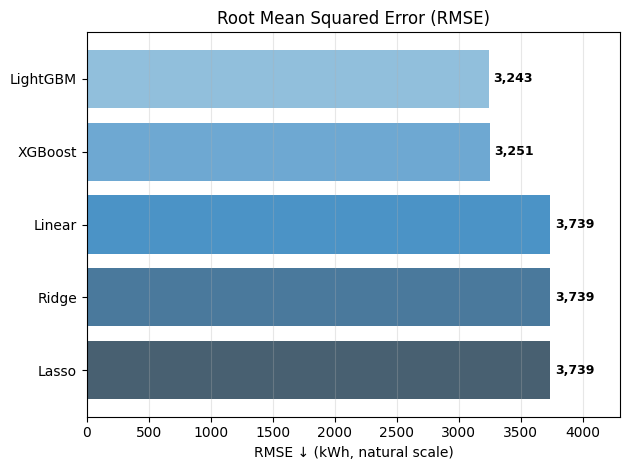
\includegraphics[width=1\columnwidth]{fig_rmse_natural.png}
    \caption{\small{RMSE on the original meter-reading scale.}}
    \label{fig:rmse_natural}
\end{subfigure}
\vspace{0.8ex}
\begin{subfigure}[t]{\columnwidth}
    \centering
    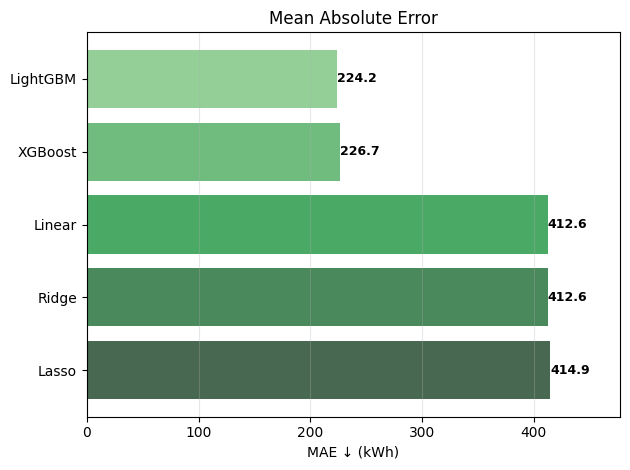
\includegraphics[width=1\columnwidth]{fig_mae_natural.png}
    \caption{\small{MAE on the original meter-reading scale.}}
    \label{fig:mae_natural}
\end{subfigure}
\caption{\small{Natural-scale error comparison. The small separation in RMSE reflects the dominance of rare extreme readings, while MAE shows that LightGBM achieves the lowest average absolute error.}}
\label{fig:rmse_mae}
\end{figure}
Fig.~\ref{fig:log_metrics} provides the key important evidence for the research question. The RMSLE plot shows a large separation between tree-based boosting models and the linear family. XGBoost and LightGBM have RMSLE values near 1.0391 and 1.0281, respectively, while Linear Regression is 1.8268, and Ridge and Lasso are 1.8268 and 1.8384, respectively.
\begin{figure}[!t]
\centering
\begin{subfigure}[t]{\columnwidth}
    \centering
    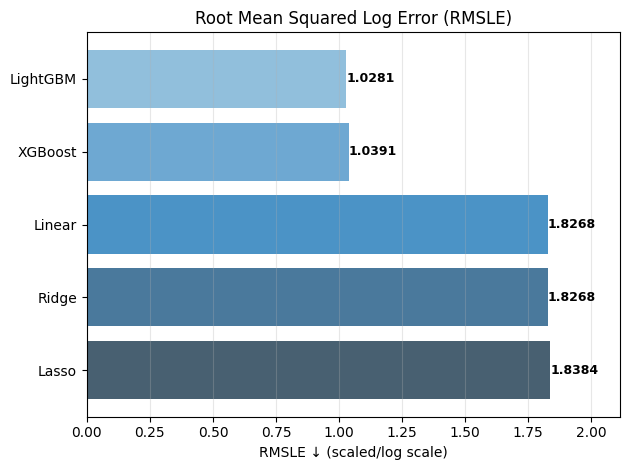
\includegraphics[width=1\columnwidth]{fig_rmsle_log.png}
    \caption{\small{RMSLE, equivalent to RMSE on $z=\log(1+y)$.}}
    \label{fig:rmsle_log}
\end{subfigure}
\vspace{0.8ex}
\begin{subfigure}[t]{\columnwidth}
    \centering
    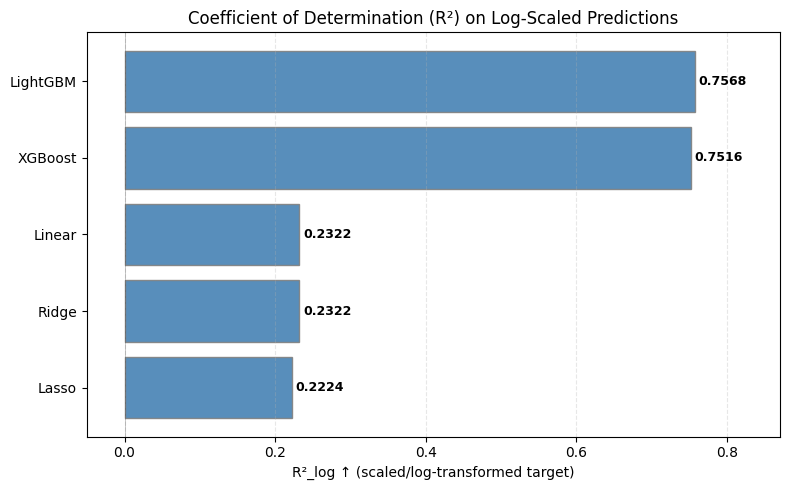
\includegraphics[width=1\columnwidth]{fig_r2_log.png}
    \caption{\small{$R^2_{\log}$ on the transformed target.}}
    \label{fig:r2_log}
\end{subfigure}
\caption{\small{Log-scale model comparison. The gradient-boosted models clearly outperform the linear and regularized linear baselines, confirming that the main learnable structure is nonlinear and interaction-dependent.}}
\label{fig:log_metrics}
\end{figure}
Fig.~\ref{fig:r2_natural} shows that natural-scale $R^2$ is close to zero for every model. This is one of the most important findings in the paper because it prevents an overly optimistic conclusion. The models do learn useful log-scale structure, but the original-scale upper tail remains difficult. Therefore, the conclusion here is that log-scale boosting captures ordinary building-energy structure, while rare extreme readings require a dedicated tail-risk modeling layer.
\begin{figure}[!t]
\centering
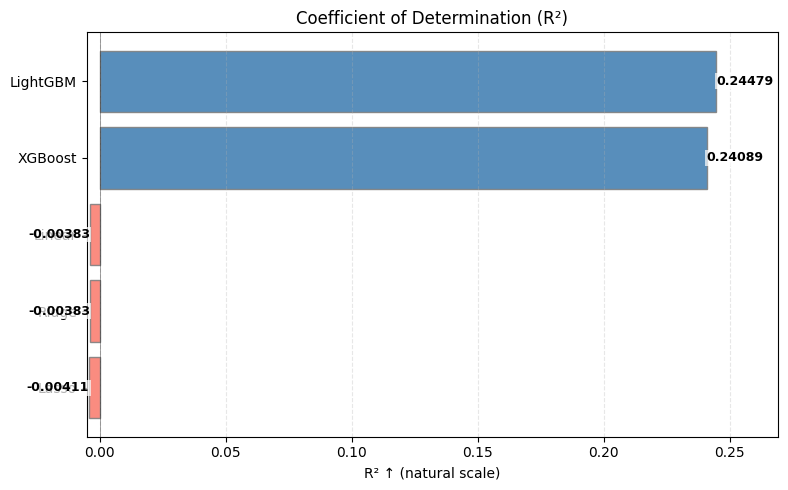
\includegraphics[width=1\columnwidth]{fig_r2_natural.png}
\caption{\small{Natural-scale $R^2$ values. Values remain near zero because rare high-consumption observations dominate the denominator and squared residual behavior on the original meter-reading scale.}}
\label{fig:r2_natural}
\end{figure}

Fig. \ref{fig:avp_log} shows the diagnostic output on logarithmic axes. The improvement in the boosted models becomes much clearer. Both XGBoost and LightGBM align more closely with the one-to-one line than the linear models, confirming that nonlinear tree ensembles capture the central structure of the transformed target more effectively. The dispersion that remains indicates that additional features, meter-specific models, lagged history, and uncertainty quantification could still improve the system.
\begin{figure*}[!t]
\centering
\begin{subfigure}[t]{0.31\textwidth}
    \centering
    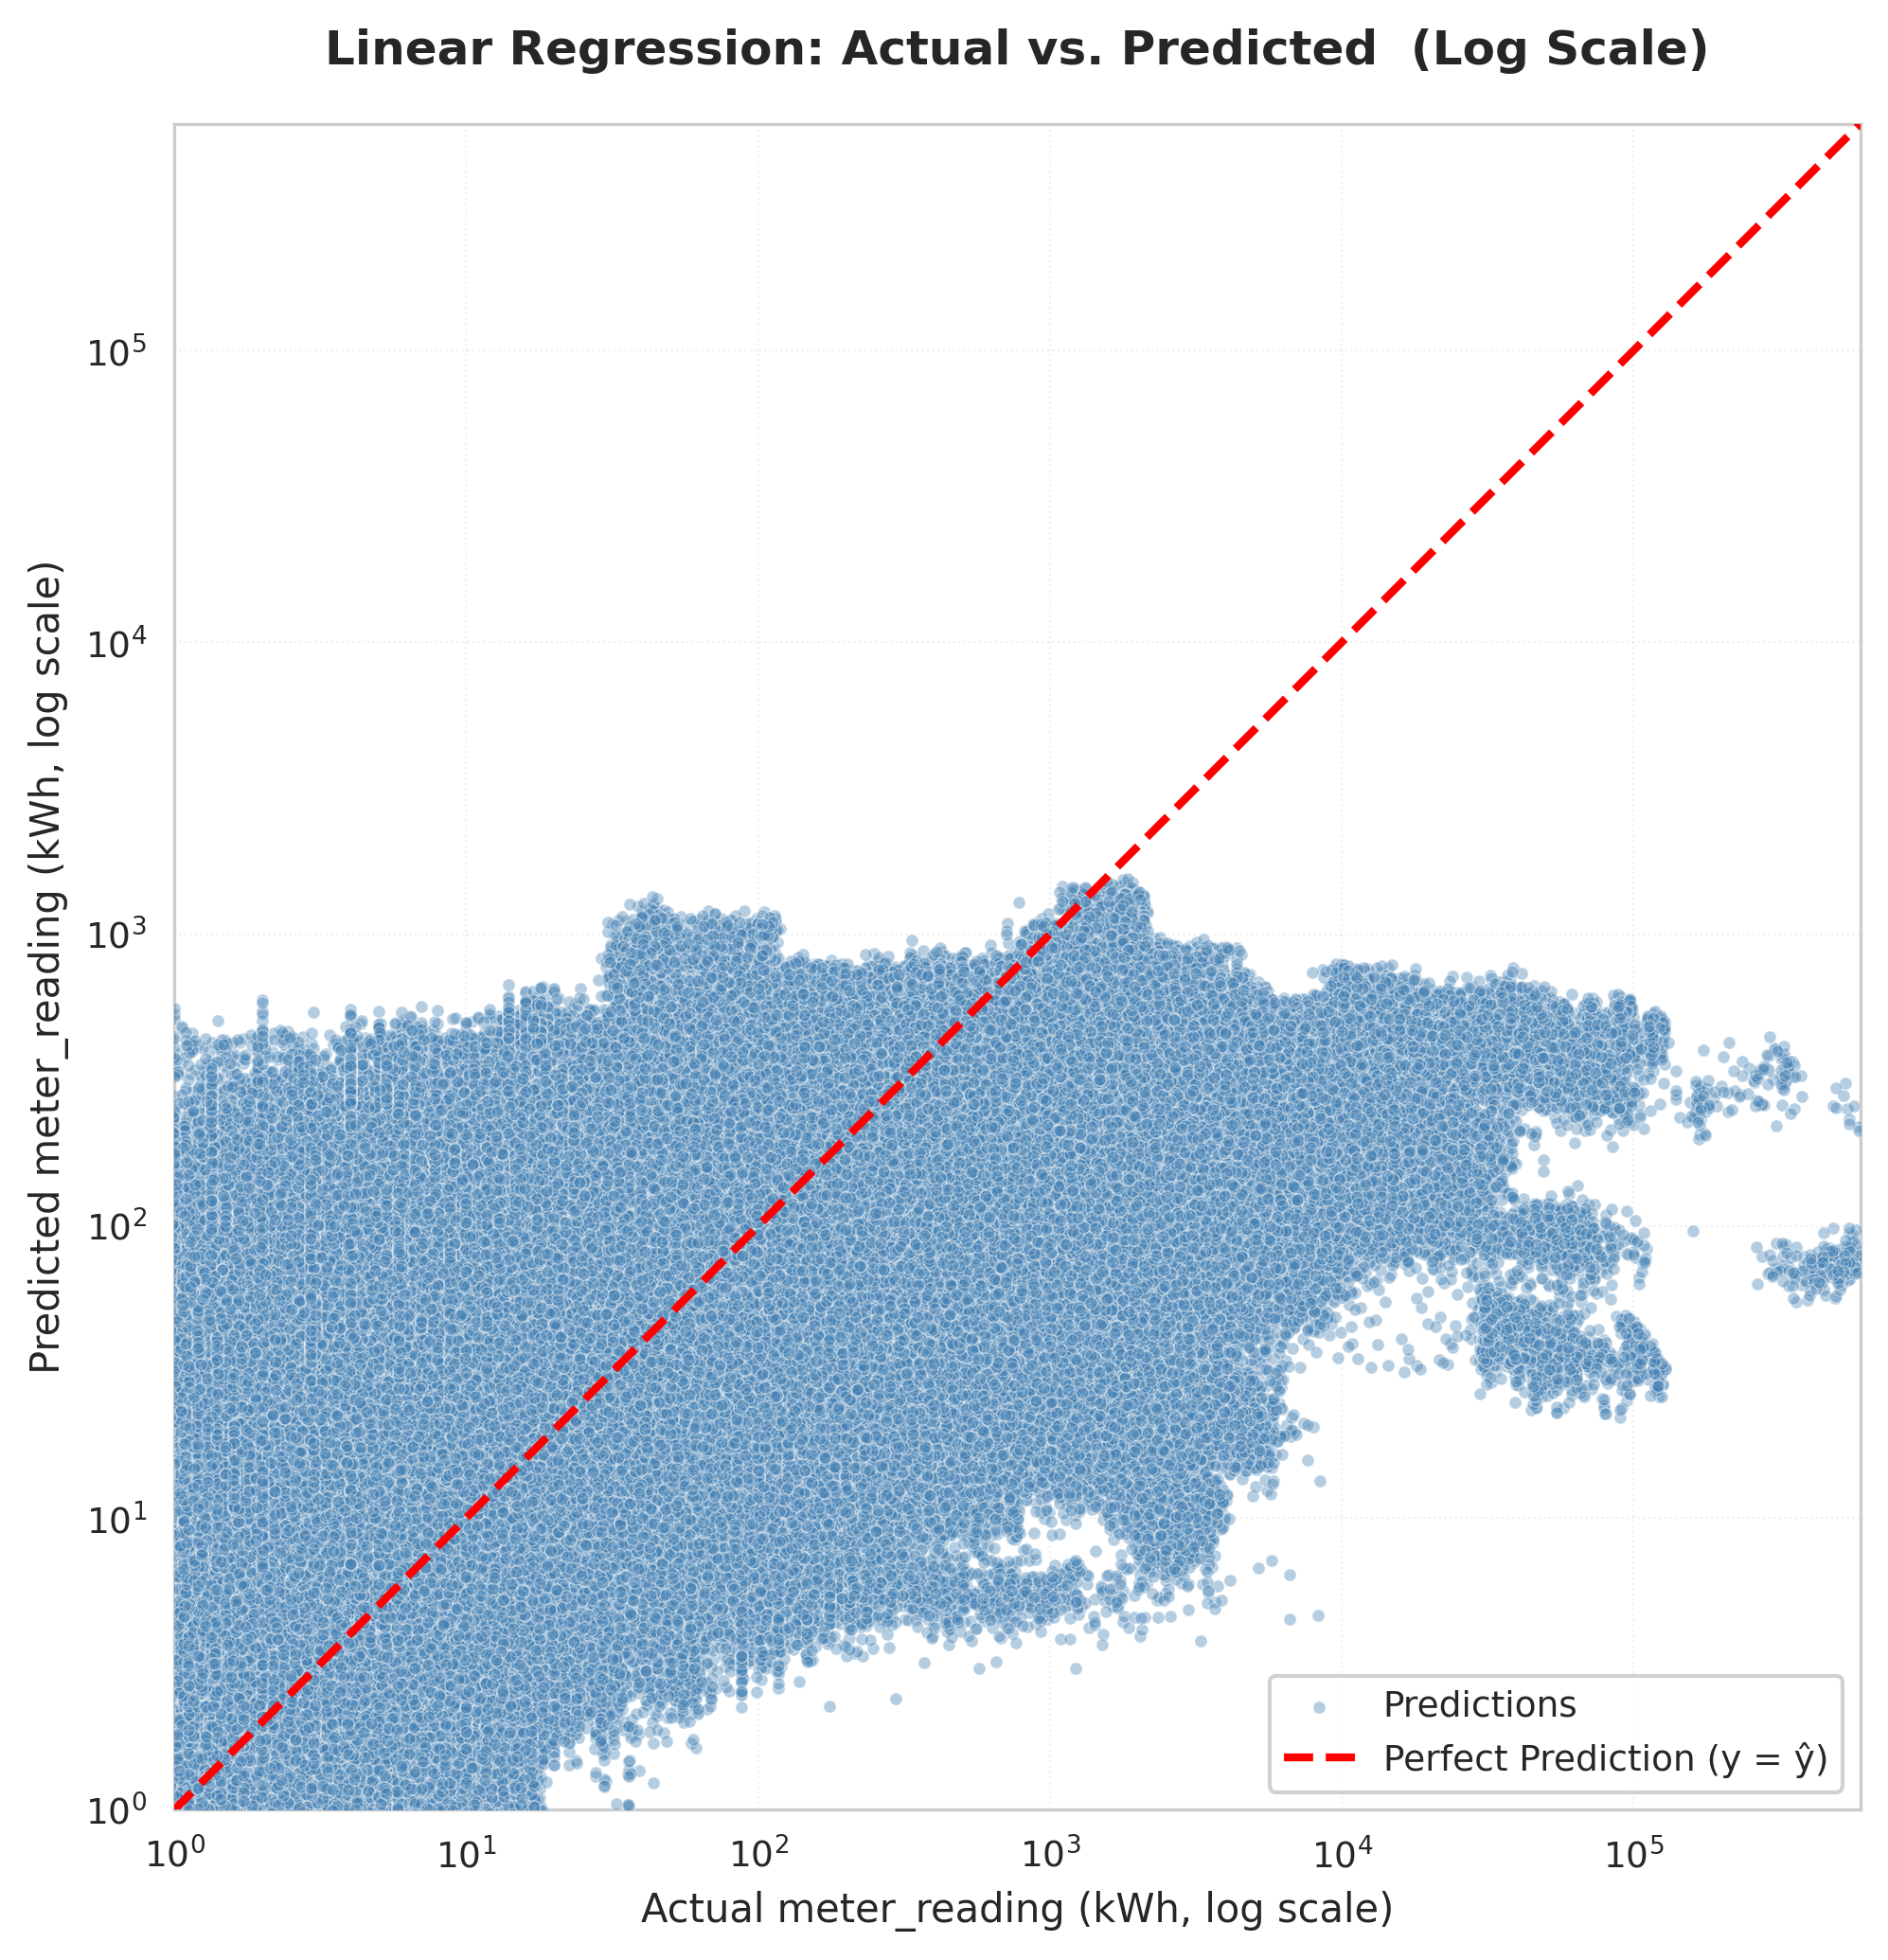
\includegraphics[width=\linewidth]{fig_avp_linear_log.png}
    \caption{\small{Linear Regression.}}
    \label{fig:avp_linear_log}
\end{subfigure}
\hfill
\begin{subfigure}[t]{0.31\textwidth}
    \centering
    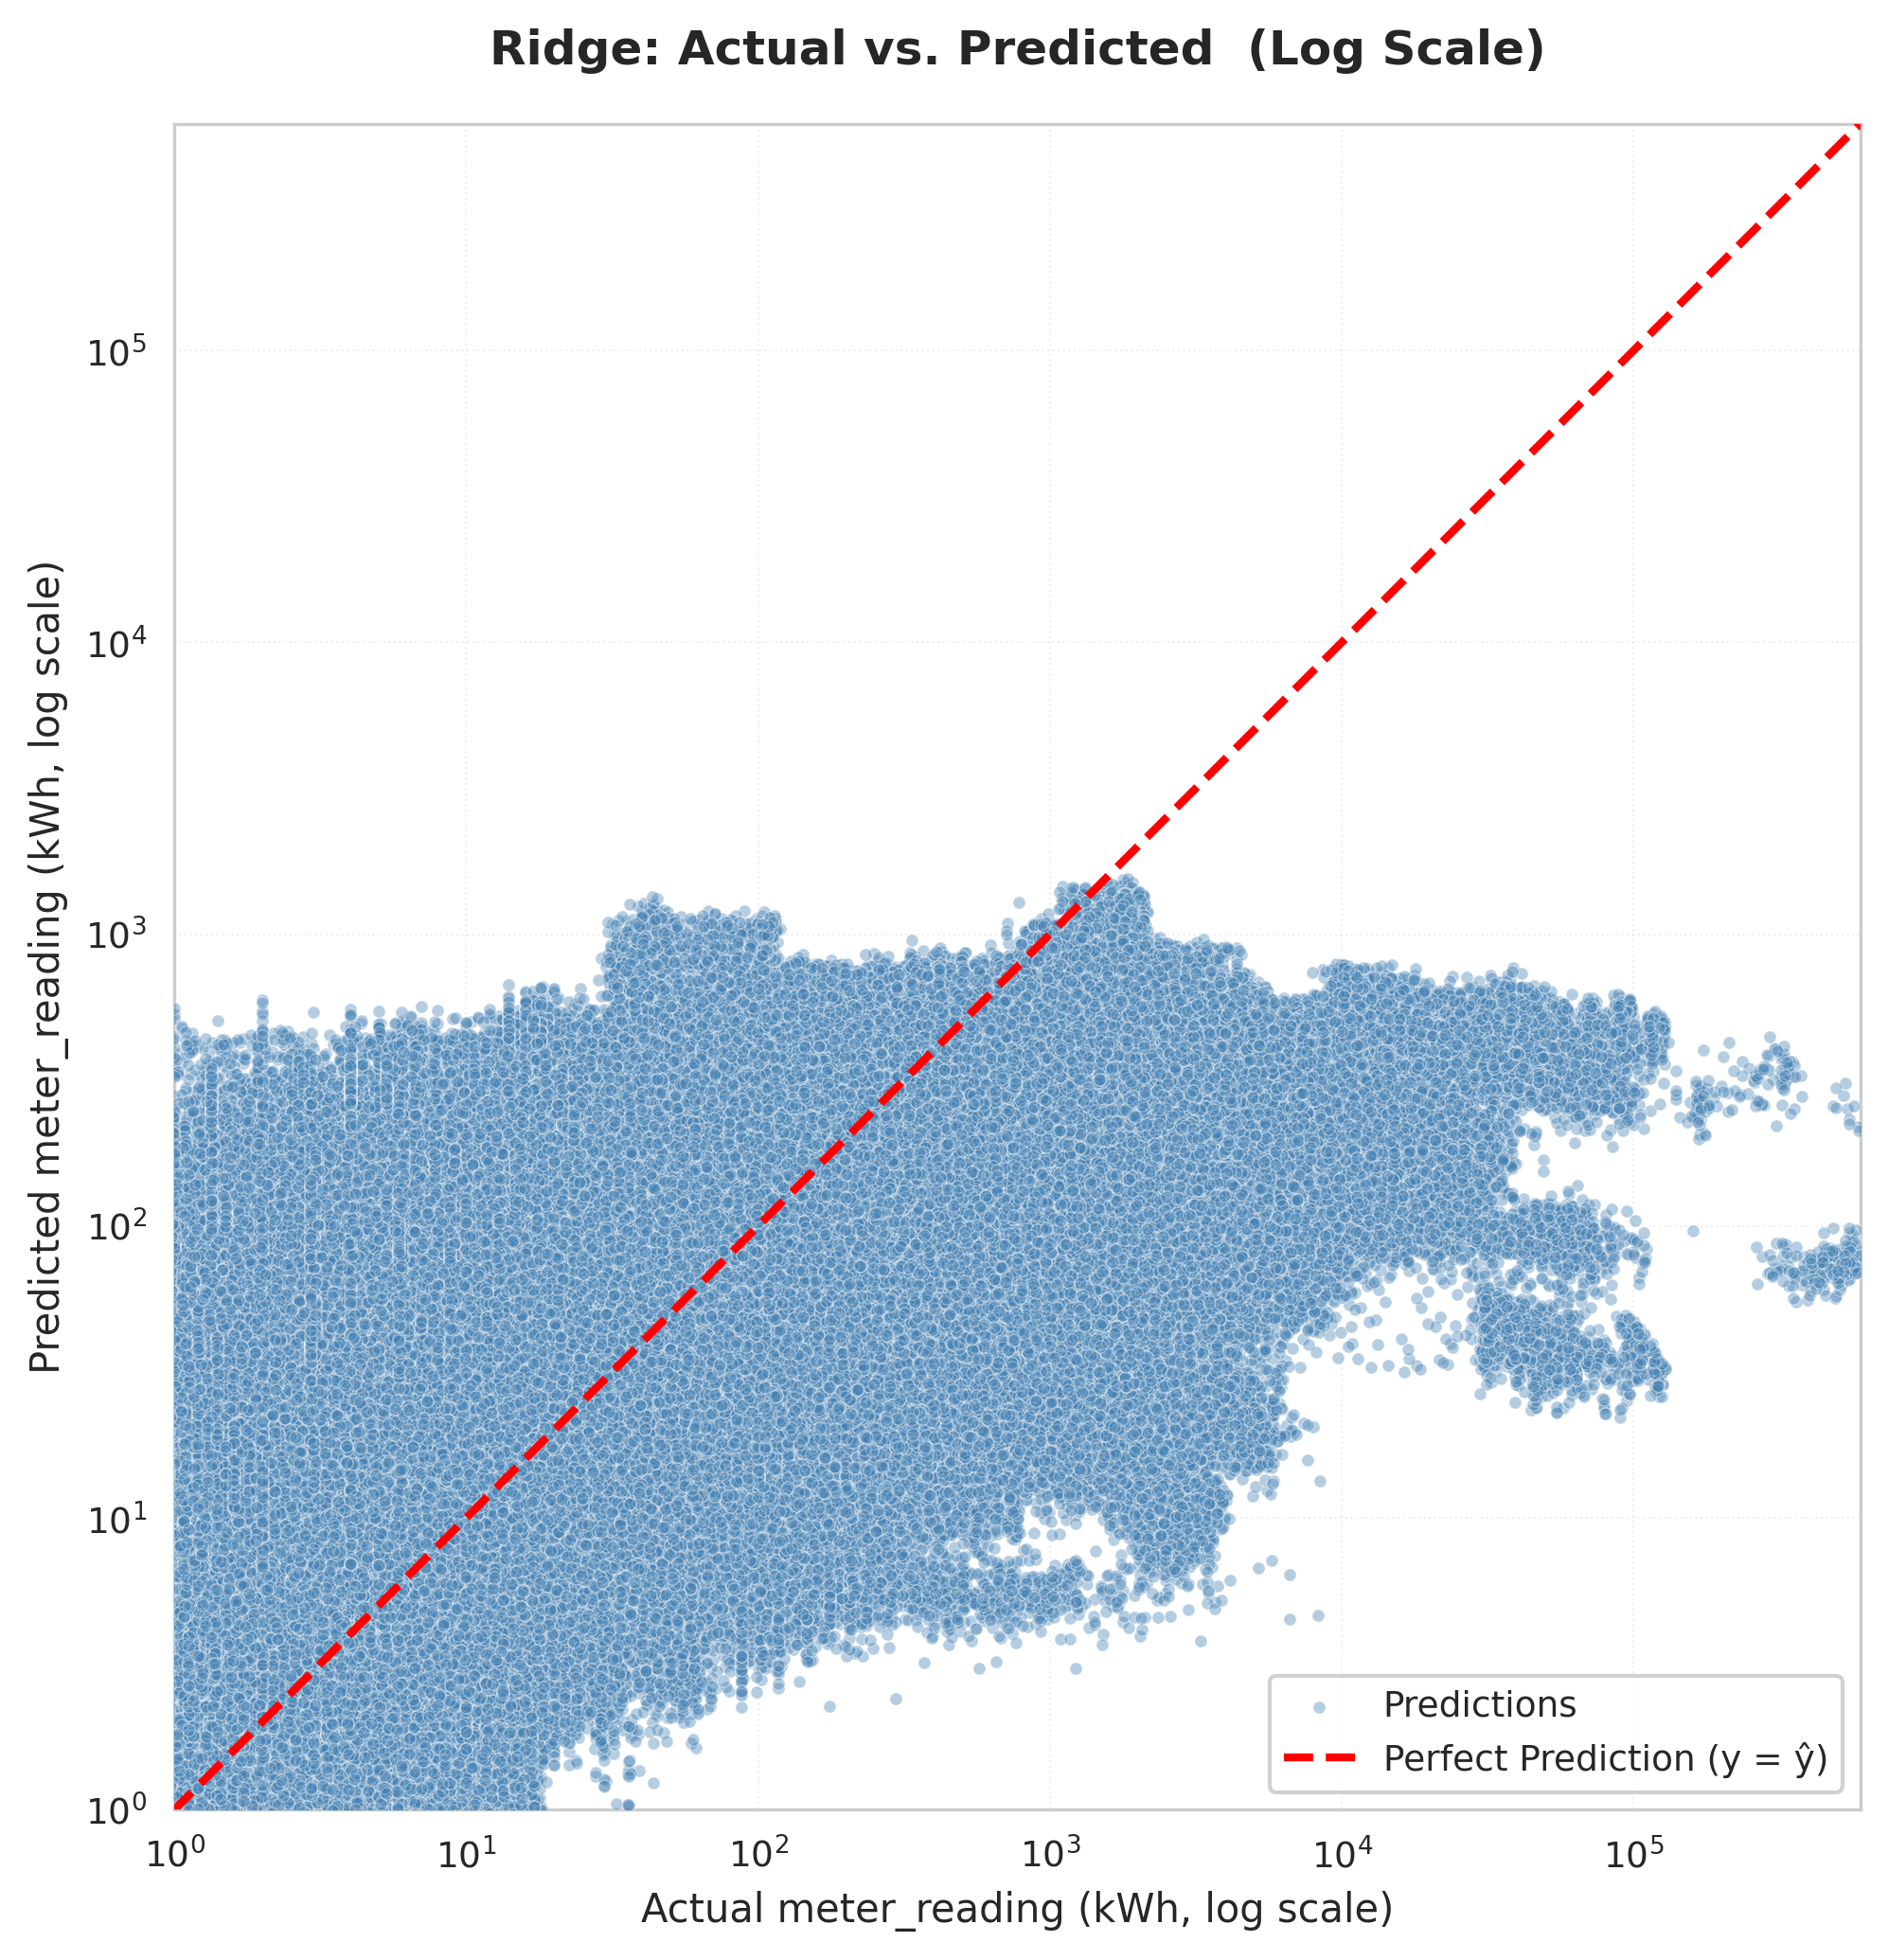
\includegraphics[width=\linewidth]{fig_avp_ridge_log.png}
    \caption{\small{Ridge.}}
    \label{fig:avp_ridge_log}
\end{subfigure}
\hfill
\begin{subfigure}[t]{0.31\textwidth}
    \centering
    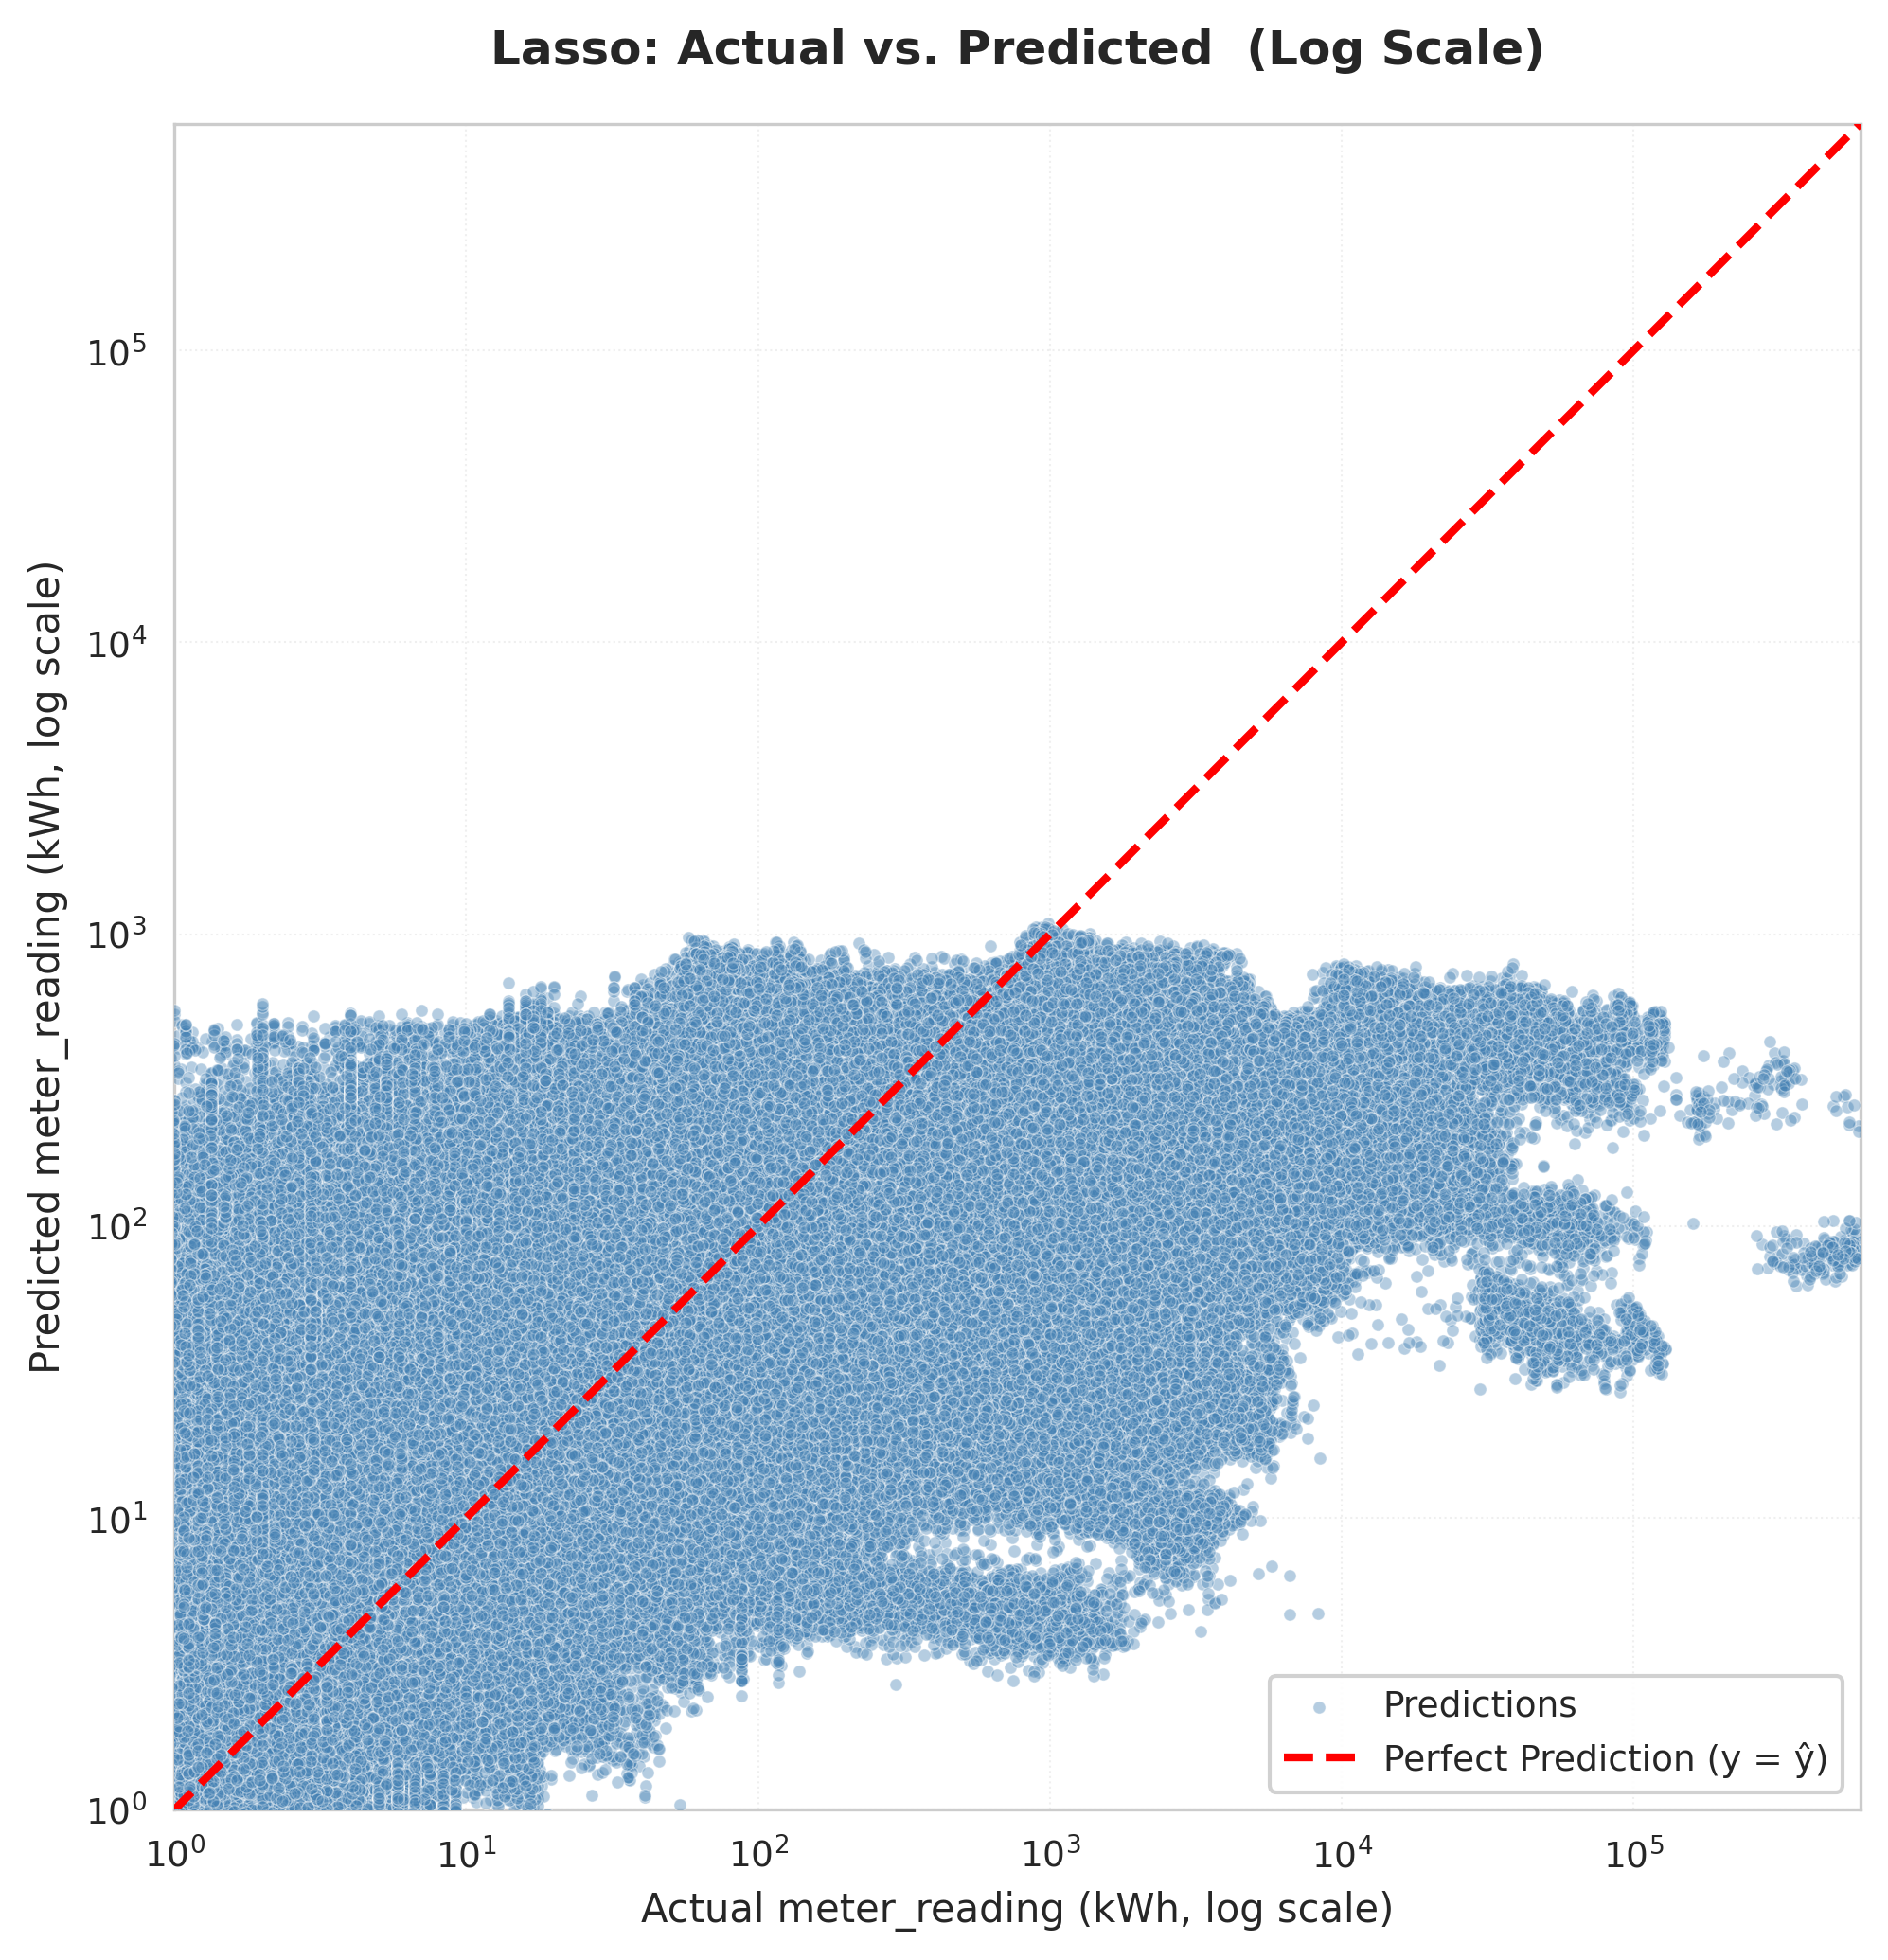
\includegraphics[width=\linewidth]{fig_avp_lasso_log.png}
    \caption{\small{Lasso.}}
    \label{fig:avp_lasso_log}
\end{subfigure}
\vspace{1ex}
\begin{minipage}{0.66\textwidth}
\centering
\begin{subfigure}[t]{0.47\textwidth}
    \centering
    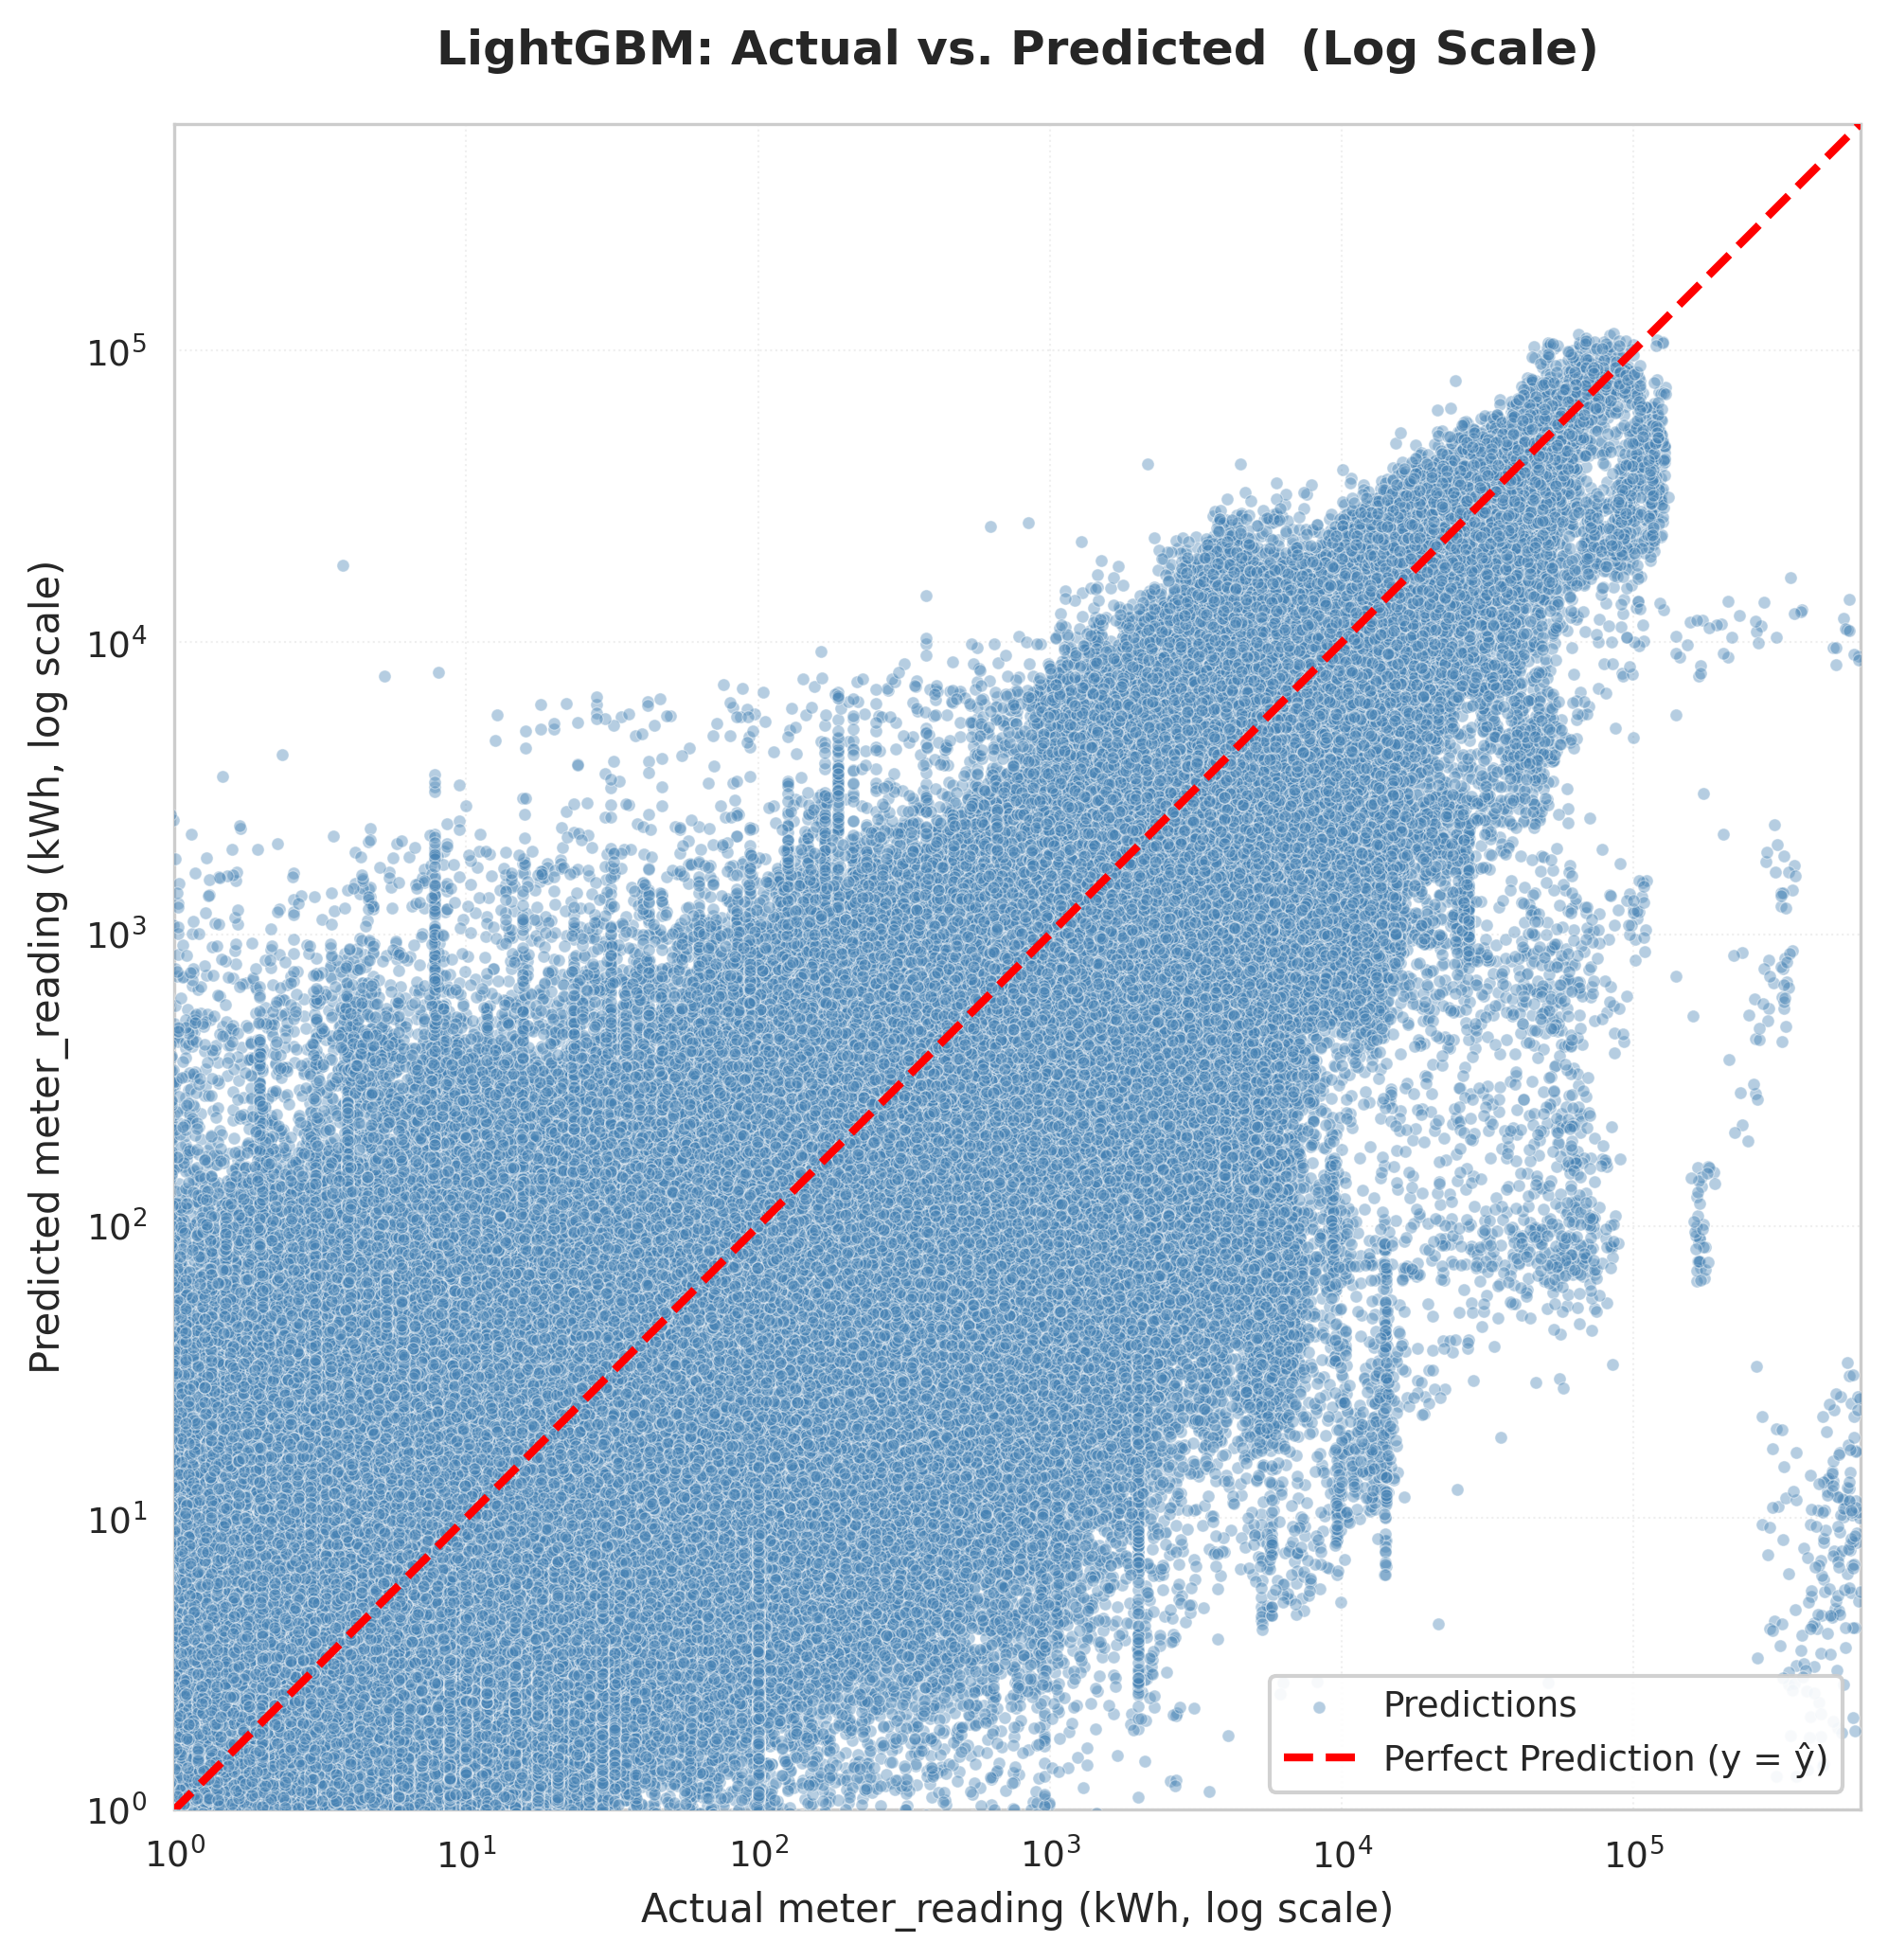
\includegraphics[width=\linewidth]{fig_avp_lightgbm_log.png}
    \caption{\small{LightGBM.}}
    \label{fig:avp_lightgbm_log}
\end{subfigure}
\hfill
\begin{subfigure}[t]{0.47\textwidth}
    \centering
    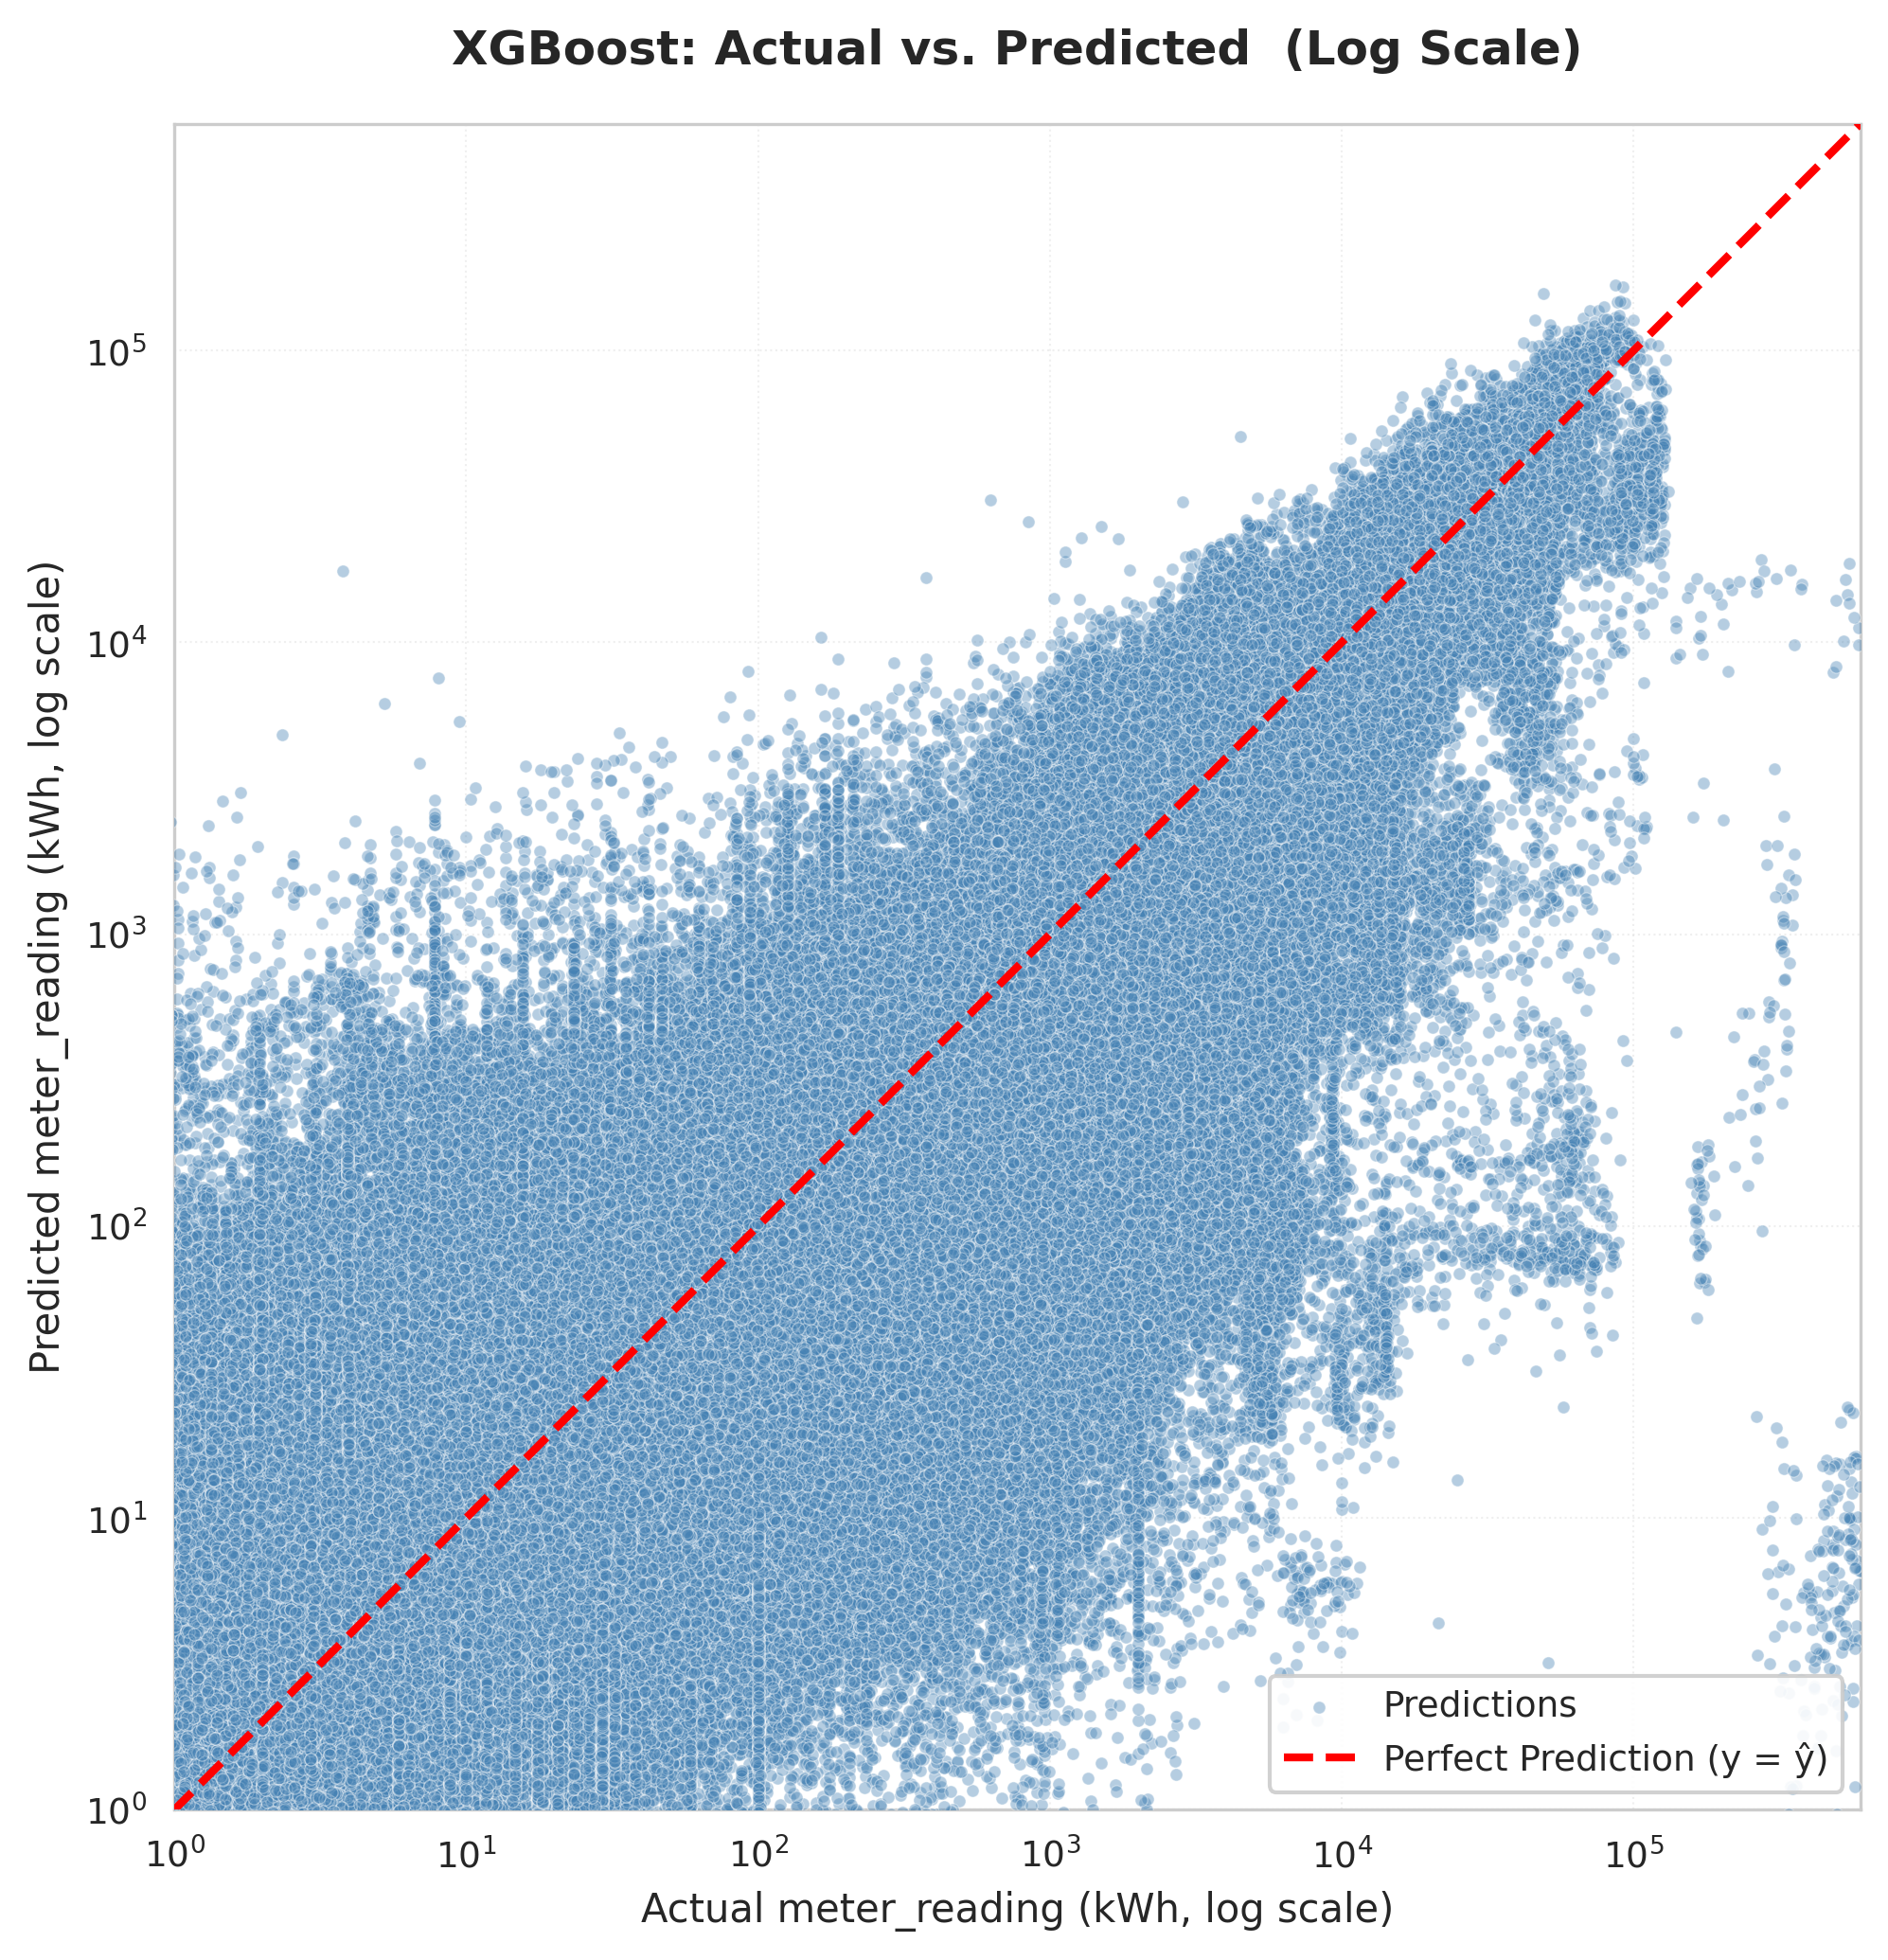
\includegraphics[width=\linewidth]{fig_avp_xgboost_log.png}
    \caption{\small{XGBoost.}}
    \label{fig:avp_xgboost_log}
\end{subfigure}
\end{minipage}
\caption{\small{Actual-versus-predicted diagnostics on logarithmic axes. The boosted models show stronger diagonal alignment than the linear-family baselines, supporting the quantitative superiority of XGBoost and LightGBM on RMSLE and $R^2_{\log}$.}}
\label{fig:avp_log}
\end{figure*}
The superiority of XGBoost and LightGBM is technically consistent with the data-generating structure of buildings. Building energy consumption is not a single smooth function of temperature or time. The effect of a weather variable can differ by site, meter type, primary use, hour, and building size. Linear regression can only represent a global additive slope unless interactions are explicitly engineered. Boosted trees, by contrast, partition the feature space into local regimes and can represent rules such as high cooling demand under one site-temperature-use combination and weak weather sensitivity under another. This explains why log-scale $R^2$ increases from 0.2322 for Linear Regression to 0.7516 for XGBoost.

The natural-scale $R^2$ values are close to zero because the original response distribution is heavy-tailed. When a few observations are extremely large, the squared-error loss becomes dominated by those observations. A model may improve the prediction of millions of ordinary readings and still appear weak under raw $R^2$ if it misses rare upper-tail events. This is not a contradiction; it is a scale effect. The interpretation is that the model captures general multiplicative structure but lacks a specialized mechanism for rare extreme readings. A practical building-energy analytics system should not rely on a single aggregate metric. A defensible deployment pipeline would use a log-scale XGBoost or LightGBM model for ordinary consumption prediction and add a second layer for tail-risk events. That second layer could include robust loss functions, quantile regression, anomaly labels, meter-specific thresholds, or prediction intervals. If the system is used for future forecasting, weather variables should be replaced by weather forecasts and lagged load features should be added to represent building inertia and recent operational state. This study has some limitations. First, it is a supervised future-period prediction study, not a complete autoregressive short-term load-forecasting system. Second, the aggregate natural-scale metrics combine different meter types, so meter-specific evaluation is needed for physical interpretation. Third, the final LightGBM model uses practical fixed settings rather than fully aligning every final parameter with the hyperparameter-search output. Fourth, the model does not provide uncertainty intervals. Fifth, interpretability tools such as SHapley Additive exPlanations (SHAP) or permutation importance are not yet included, so the present paper explains model behavior through performance metrics and diagnostic plots.

\section{Conclusion and Future Work}
This study proposed a time-aware building energy consumption prediction appraoch using machine learning. The workflow predicts hourly ASHRAE meter readings using building identifiers, meter type, site information, weather variables, calendar variables, log-transformed square footage, and primary-use encoding. A log-target formulation was derived and justified analytically, and five models were compared under a chronological validation protocol. The results show that XGBoost is the strongest overall model, achieving RMSLE of 1.0391 and $R^2_{\log}$ of 0.7516, while LightGBM is a very close alternative and gives the lowest MAE. Linear Regression, Ridge, and Lasso are useful baselines, but they do not capture enough nonlinear and interaction-dependent structure.

Furthermore, a target scale determines interpretation. On the log scale, gradient boosting reveals substantial learnable structure in the ASHRAE data. On the original meter-reading scale, rare extreme values dominate squared-error behavior and keep $R^2$ close to zero. Therefore, the best practical conclusion is not simply that one model performs better than the others, but that log-scale boosting should be paired with a future tail-risk layer. Future work will focus on adding lagged meter readings and horizon-specific targets, building meter-specific or building-cluster models, evaluating weather-ablation experiments, optimize robust or quantile losses for extremes, produce calibrated prediction intervals, and use explainability methods to quantify which building, weather, and calendar variables drive predictions.










\bibliographystyle{IEEEtran}
\bibliography{References}

\end{document}
